% coding:utf-8

%FOSASTOC, a LaTeX-Code for a electrical summary of stochastic
%Copyright (C) 2013, Daniel Winz, Ervin Mazlagic

%This program is free software; you can redistribute it and/or
%modify it under the terms of the GNU General Public License
%as published by the Free Software Foundation; either version 2
%of the License, or (at your option) any later version.

%This program is distributed in the hope that it will be useful,
%but WITHOUT ANY WARRANTY; without even the implied warranty of
%MERCHANTABILITY or FITNESS FOR A PARTICULAR PURPOSE.  See the
%GNU General Public License for more details.
%----------------------------------------

\chapter{Diskrete Verteilungen}
Diskrete Verteilungen beschreiben Probleme, welche
Ergebnisse aus $\mathbb{N}$ liefern und binär sind.

\paragraph{Binär}
\gls{Binaer} bedeutet, dass ein Ereignis zwei Werte annehmen kann. Bekannte
Beispiele binärer Probleme sind
\begin{itemize}
	\item Gewinnlose \hfill{} (\emph{Gewinn, Zonk})
	\item Münzwurf \hfill{} (\emph{Kopf, Zahl})
	\item Telefon \hfill{} (\emph{klingelt, klingelt nicht})
\end{itemize}
Viele nicht-binäre Probleme können aber leicht in binäre gewandelt
werden. Beispielsweise liefert ein Sensor analoge Signale, diese sind
$\notin \mathbb{N}$ noch sind diese binär. 
Dennoch kann man das Signal binär
untersuchen mit der Fragestellung 
"`\emph{Ist der Wert grösser als $xy$?}"'.
Diese Frage kann semantisch nur mit \emph{Ja} und \emph{Nein} beantwortet
werden und beschreibt somit ein binäres Problem. Die Zahl der Antworten
kann wiederum nur $\in \mathbb{N}$ sein. Somit sind die Bedingungen 
für ein binäres Problem gegeben.

\newpage
\section{Hypergeometrische Verteilung}
Die hypergeometrische Verteilung entspricht dem \gls{Urnenmodell}:
\begin{itemize}
	\item Urne hat $r$ rote (postive) und $s$ schwarze (negative)
		Kugeln
		\[ r,s \in \mathbb{N} \]
	\item Die Menge der roten als auch der schwarzen Kugeln ist fix 
		\[ r,s \neq \infty \]
	\item Ein erzieltes Ergebnis reduziert die entsprechende Menge
		(\emph{Ziehen ohne Zurücklegen})
		\[ r \rightarrow  R - 1\]
\end{itemize}

\subsection{Verteilungsfunktion}
\[  
	X \sim Hyp(n,r,s)
\]

\[ \begin{array}{c l}
	n & \text{Anzahl Ziehungen} \\
	r & \text{Anzhal roter Kugeln (positive Ereignisse)} \\
	s & \text{Anzahl blauer Kugeln (negative Ereignisse)} \\
	N & \text{Anzahl Kugeln in der Urne } (N=r+s)
\end{array} \]

\[
	P(X=k)
		= \frac{\displaystyle 
			\binom{r}{k} \cdot \binom{s}{n-k}}{
				\displaystyle \binom{r+s}{n}}
		= \frac{\displaystyle 
			\binom{r}{k} \cdot \binom{N-r}{n-k}}{
				\displaystyle \binom{N}{n}}
\]

\subsection{Erwartungswert}

\[ 
	E(X) = n \cdot \frac{r}{N}, \qquad X \sim Hyp(n,r,s)
\]

\subsection{Varianz}

\[  
	Var(X) = n \cdot \frac{r}{N} \cdot 
		\left(1 - \frac{r}{N} \right)
		\cdot \frac{N-n}{N-1}, \qquad X \sim Hyp(n,r,s)
\]

\subsection{Verwendung in R}
\lstinline{R} stellt grundsätzlich vier Funktionen für die 
hypergeometrische Verteilung zur Verfügung. 
\begin{itemize}
	\item \lstinline{dhyper()} \hfill{} 
		(\emph{Wahrscheinlichkeitsverteilung})
	\item \lstinline{phyper()} \hfill{}
		(\emph{kumulative Wahrscheinlichkeit})
	\item \lstinline{qhyper()} \hfill{}
		(\emph{Verteilung der Quantile})
	\item \lstinline{rhyper()} \hfill{}
		(\emph{Zufallszahlen})
\end{itemize}
Die Abbildung \ref{fig:hyper} zeigt jeweils einen Plot zu den gegebenen
Funktionen aus \lstinline{R}. Für weitere Informationen zu Plots siehe
Kapitel \ref{sec:plots}.





\begin{figure}[h!]
\centering
\begin{subfigure}[b]{0.48\textwidth}
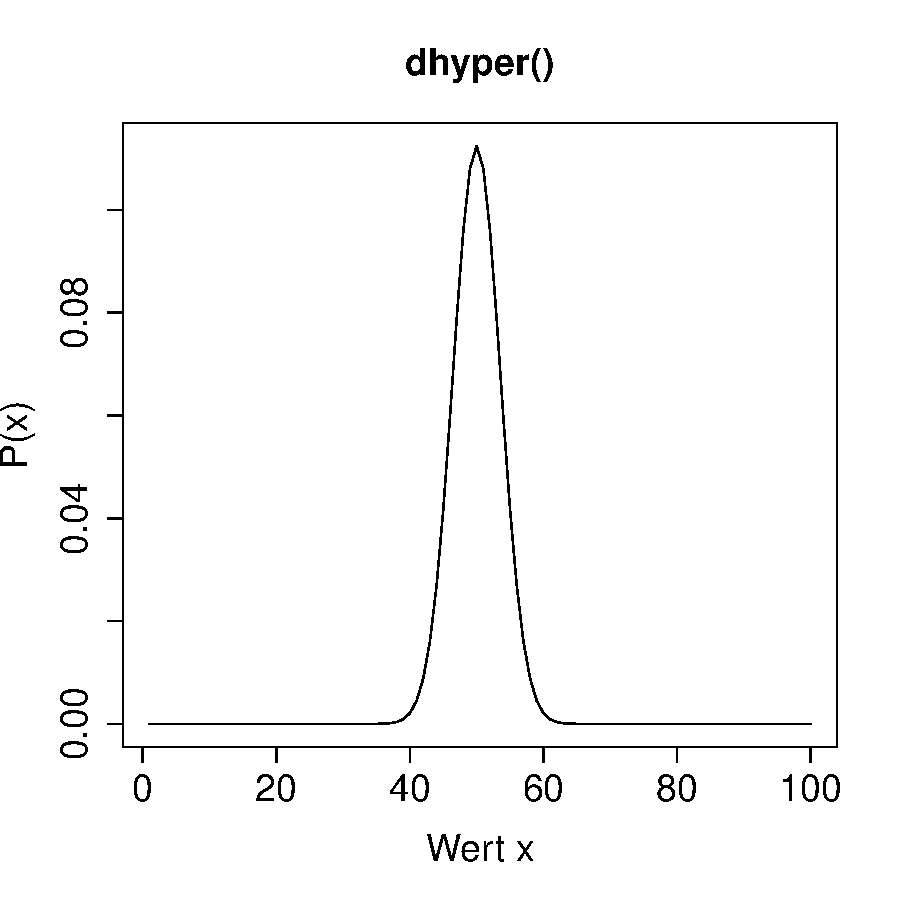
\includegraphics{verteilungen-005}
\caption{Wahrscheinlichkeitsverteilung}
\end{subfigure}
\begin{subfigure}[b]{0.48\textwidth}
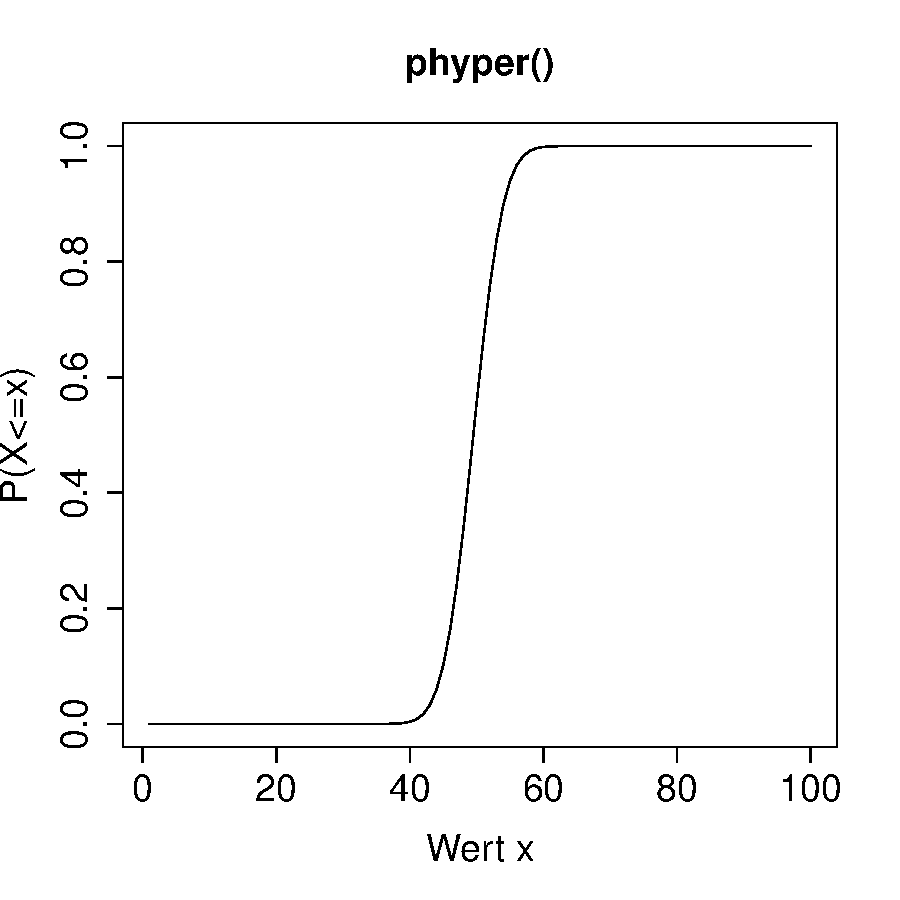
\includegraphics{verteilungen-006}
\caption{kumulative Wahrscheinlichkeit}
\end{subfigure}

\begin{subfigure}[b]{0.48\textwidth}
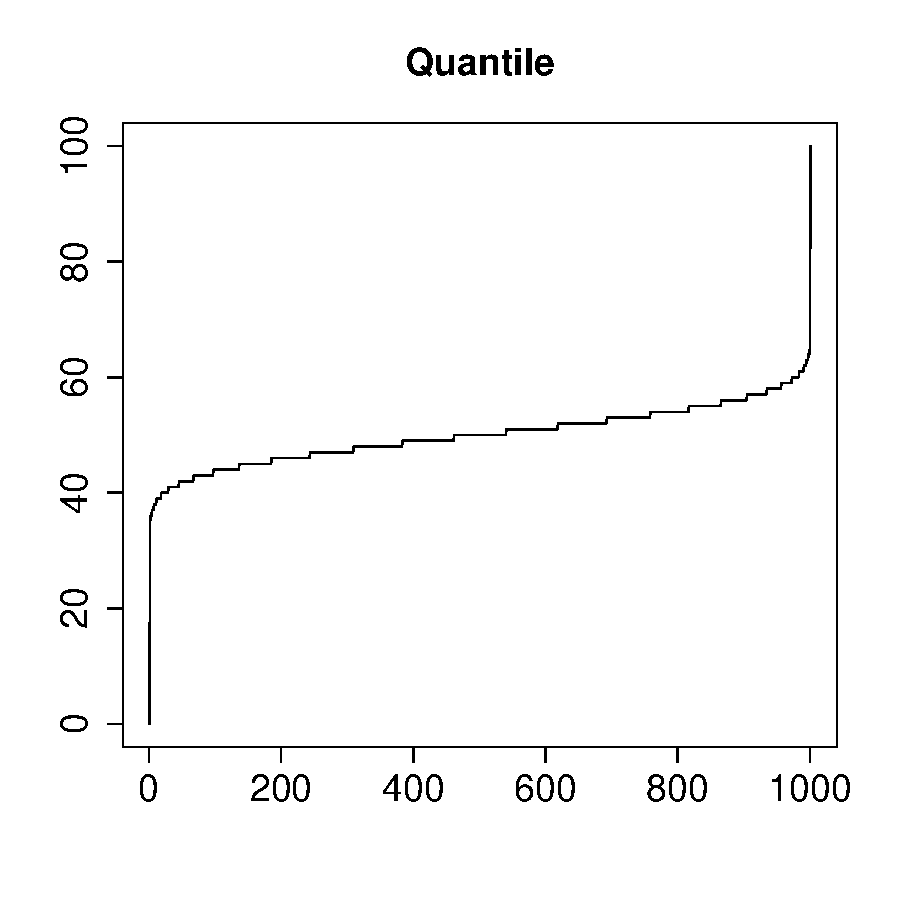
\includegraphics{verteilungen-007}
\caption{Quantile}
\end{subfigure}
\begin{subfigure}[b]{0.48\textwidth}
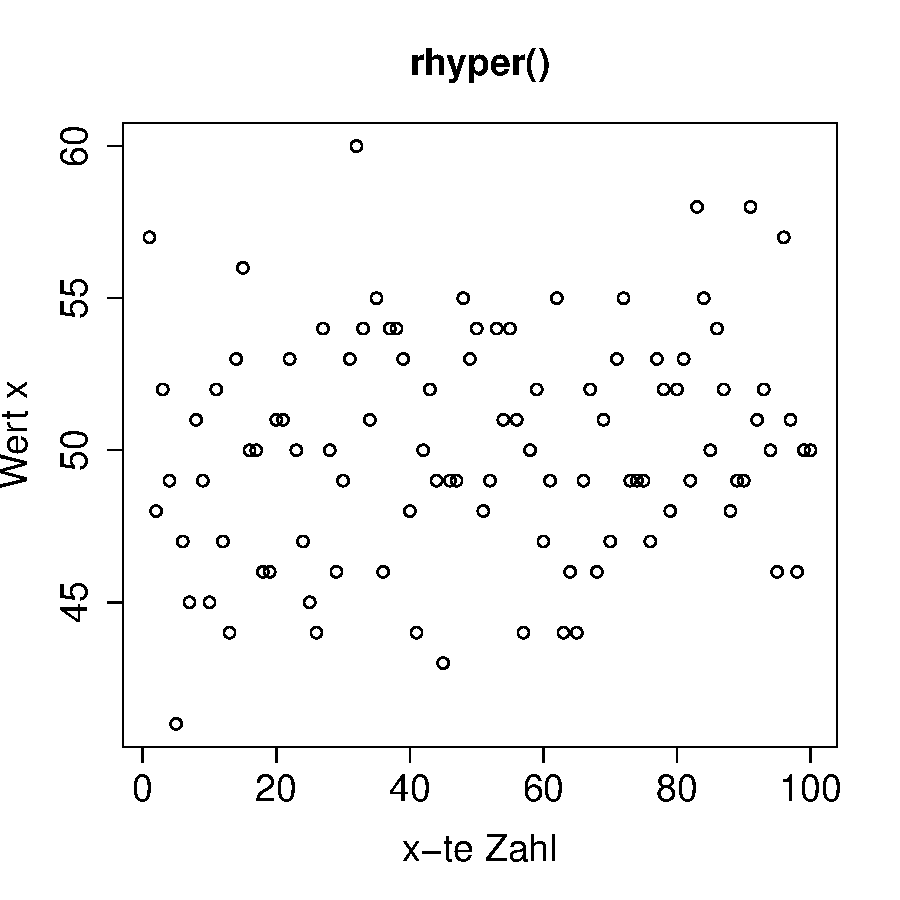
\includegraphics{verteilungen-008}
\caption{Zufallszahlen}
\end{subfigure}
\caption{Hypergeometrische Verteilung ($m=100, n=100, k=100$)}
\label{fig:hyper}
\end{figure}

\clearpage

\subsection{Beispiel einer hypogeometrischen Verteilung}
Ein Beispiel aus dem Alltag ist die Teambildung im Mannschaftssport.
Ein Turnverein hat $9$ männliche und $17$ weibliche Mitglieder. Für ein
Fussballmatch gegen einen anderen Verein muss nun ein Team mit $11$
Mitgliedern gebildet werden. Wie wahrscheinlich ist es, dass das
Team aus einer bestimmten Anzahl Männern oder Frauen besteht?
\paragraph{Berechnung in R}
\begin{Schunk}
\begin{Sinput}
> man <- 9; women <- 17; player <- 11
> boys <- dhyper(x=c(1:player), m=man, n=women, k=player)
> girls <- dhyper(x=(1:player), m=women, n=man, k=player)
> plot(boys, type='h')
> plot(girls, type='h')
\end{Sinput}
\end{Schunk}
\begin{figure}[h!]
\centering
\begin{subfigure}[b]{0.48\textwidth}
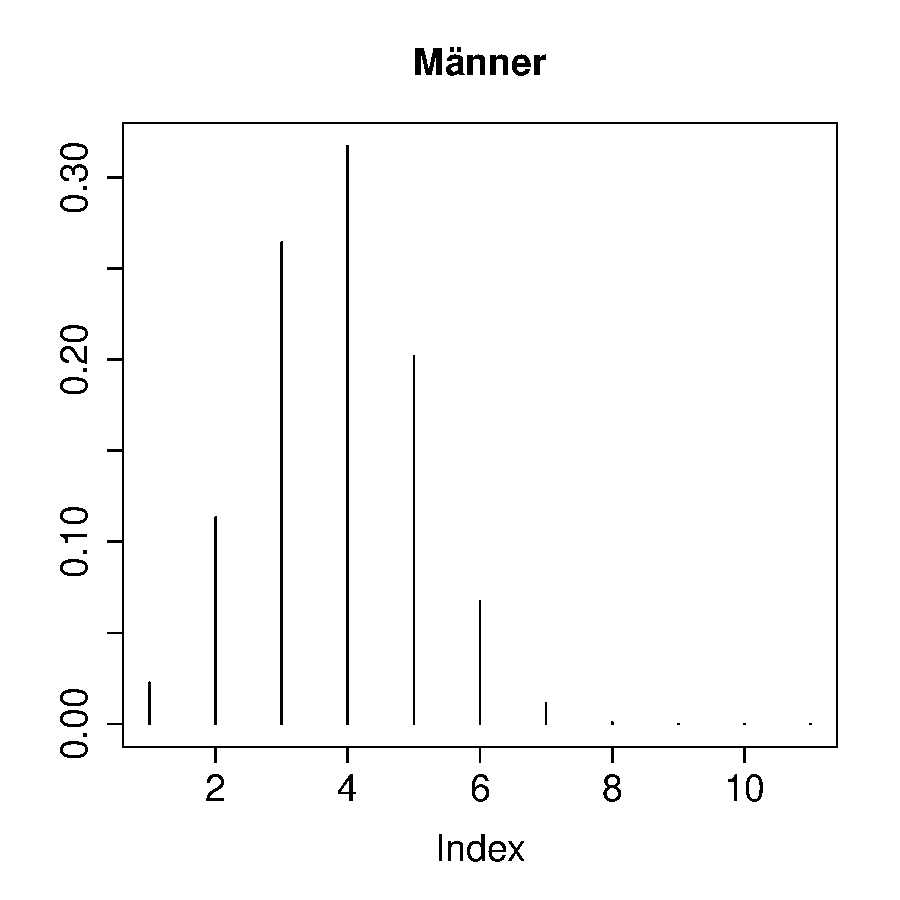
\includegraphics{verteilungen-012}
\caption{$P(x)$ der Männer im Team}
\end{subfigure}
\begin{subfigure}[b]{0.48\textwidth}
\centering
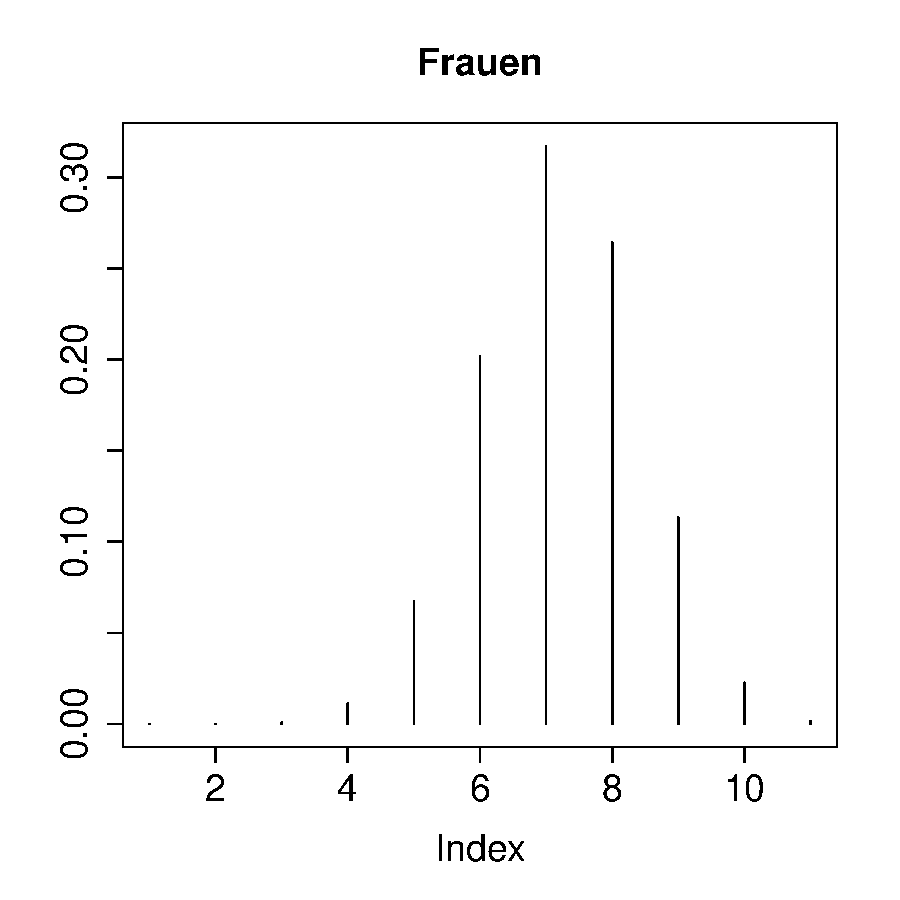
\includegraphics{verteilungen-013}
\caption{$P(x)$ der Frauen im Team}
\end{subfigure}
\caption{Teambildung nach Geschlecht}
\label{fig:team}
\end{figure}

\noindent
Die Plots aus der Abbildung \ref{fig:team} zeigen, dass es mit der 
höchsten Wahrscheinlichkeit
4 Männer und 7 Frauen im Team hat, was die gewünschte Anzahl von Spielern
ergibt für das Team ($4+7=11$). 

\clearpage
\newpage
\section{Binomialverteilung}
Die Binomialverteilung ist eine Verteilung, welche bei binären Problemen
auftritt wobei ein erzieltes Ergebnis nicht die weiteren Ergebnisse
beeinflusst. Sie ist somit ein Grenzfall der hypergeometrischen 
Verteilung (nämlich dann, wenn es sehr viele rote und schwarze 
Kugeln gibt).
\[ 
	\lim_{r,s \rightarrow \infty} Hyp(n,r,s) 
	\quad \Rightarrow \quad Bin(n,p)
\]

\subsection{Verteilungsfunktion}

\[ 
	X \sim Bin(n,p)
\]

\[ \begin{array}{c l} 
	n & \text{Anzahl Versuche} \\
	p & \text{Trefferwahrscheinlichkeit}
\end{array} \]

\[ \begin{array}{l c l} 
	P(X=x)
		&= 
		& \displaystyle \binom{n}{x} \cdot p^x 
			\cdot (1-p)^{n-x} \\
	& & \\
		&= 
		& \frac{\displaystyle n!}{\displaystyle x!\, (n-x)!} 
			\cdot p^x \cdot (1-p)^{n-x}
\end{array} \]

\subsection{Addition}
Mit dem Additionsgesetz für stochastisch unabhängige Zufallsvariablen 
können auch binomiaverteilte Zufallsvariablen, welche die gleiche
Eintrittswahrscheinlichkeit $p$ haben, zusammengefasst werden.
\[  
	\left.\begin{array}{l l }
		X \sim Bin(n_1, p) & \\
		& \\
		Y \sim Bin(n_2, p) & \\
	\end{array} \right\}
	\Rightarrow (X+Y) \sim Bin((n_1 + n_2), p)
\]

\subsection{Erwartungswert}

\[  
	E(X) = n \cdot p, \qquad X \sim Bin(n,p)
\]


\subsection{Varianz}

\[  
	Var(X) = n \cdot p \cdot (1-p), \qquad X \sim Bin(n,p)
\]

\subsection{Verwendung in R}
\lstinline{R} stellt grundsätzlich vier Funktionen für die 
Binomialverteilung zur Verfügung. 
\begin{itemize}
	\item \lstinline{dbinom()} \hfill{} 
		(\emph{Wahrscheinlichkeitsverteilung})
	\item \lstinline{pbinom()} \hfill{}
		(\emph{kumulative Wahrscheinlichkeit})
	\item \lstinline{qbinom()} \hfill{}
		(\emph{Verteilung der Quantile})
	\item \lstinline{rbinom()} \hfill{}
		(\emph{Zufallszahlen})
\end{itemize}
Die Abbildung \ref{fig:binom} zeigt jeweils einen Plot zu den gegebenen
Funktionen aus \lstinline{R}. Für weitere Informationen zu Plots siehe
Kapitel \ref{sec:plots}.





\begin{figure}[h!]
\centering
\begin{subfigure}[b]{0.48\textwidth}
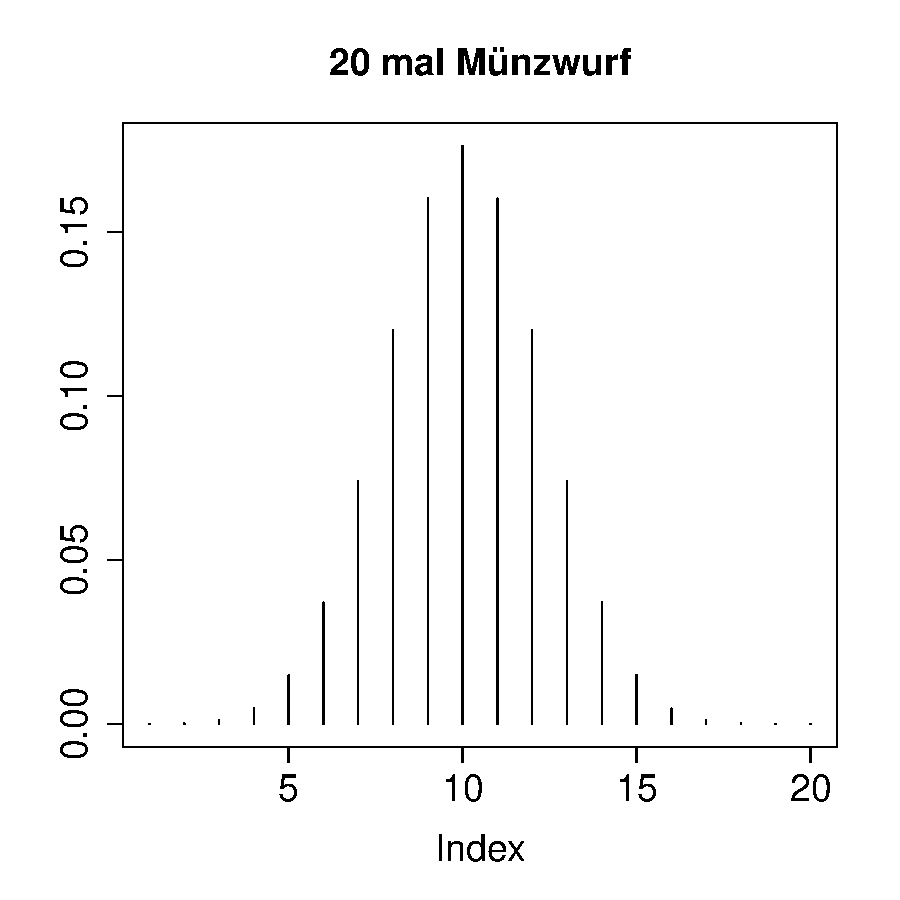
\includegraphics{verteilungen-018}
\caption{Wahrscheinlichkeitsverteilung}
\end{subfigure}
\begin{subfigure}[b]{0.48\textwidth}
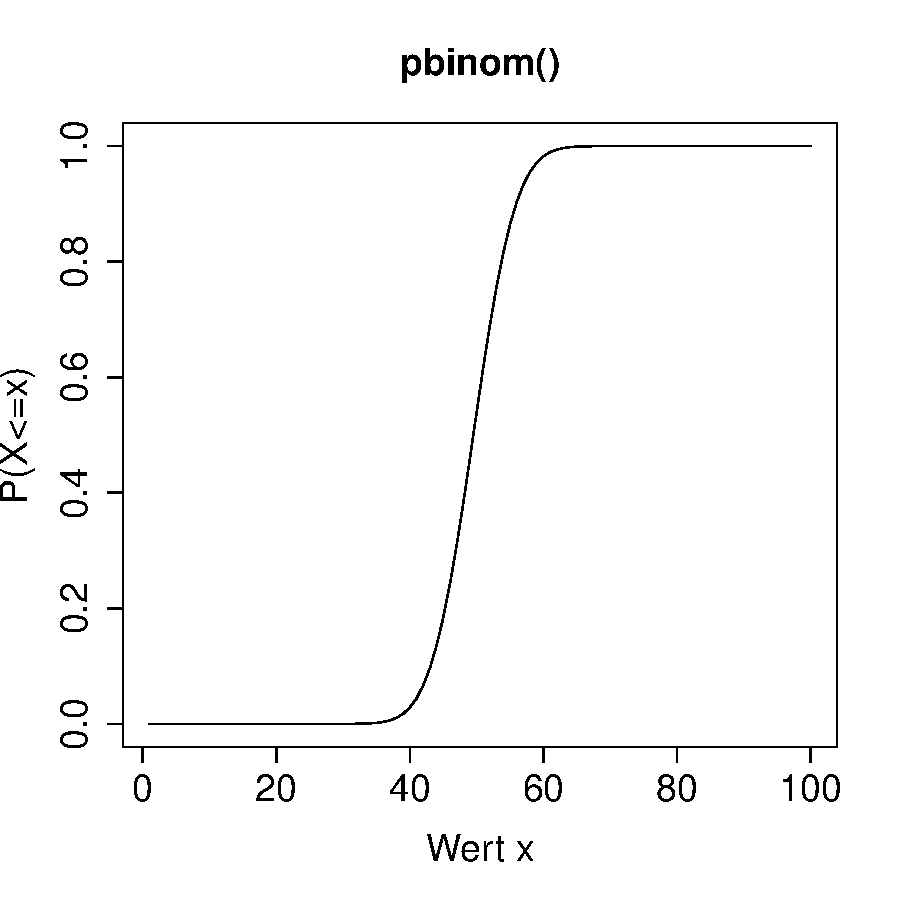
\includegraphics{verteilungen-019}
\caption{kumulative Wahrscheinlichkeit}
\end{subfigure}

\begin{subfigure}[b]{0.48\textwidth}
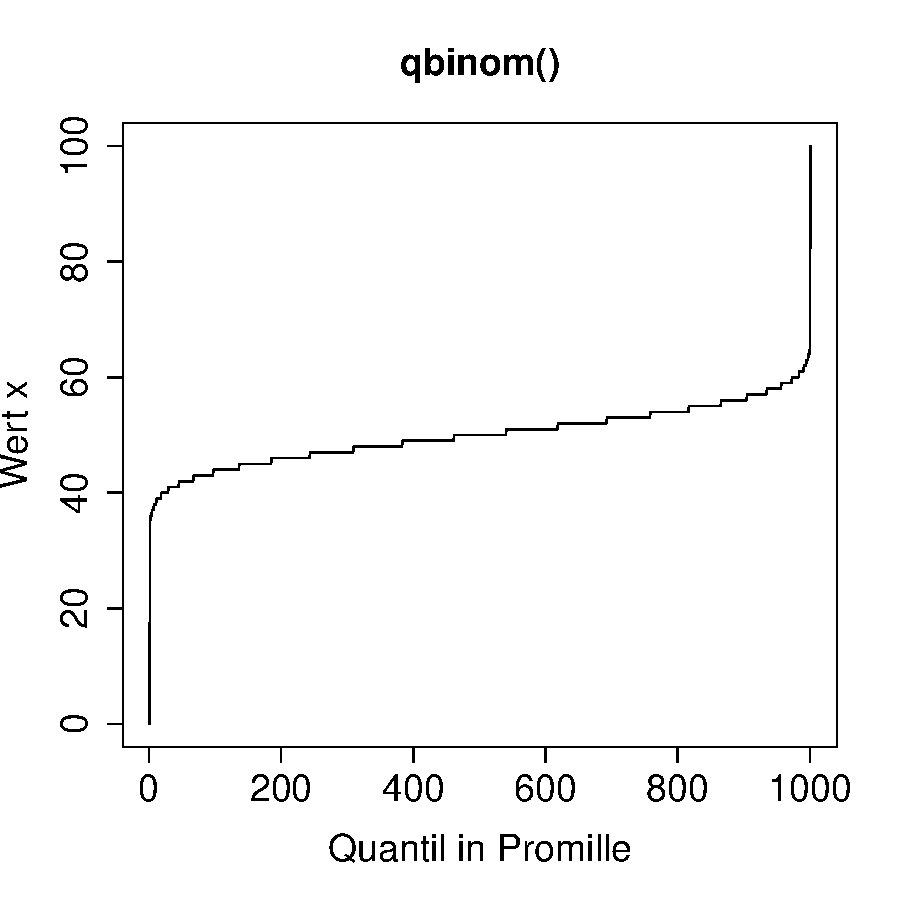
\includegraphics{verteilungen-020}
\caption{Quantile}
\end{subfigure}
\begin{subfigure}[b]{0.48\textwidth}
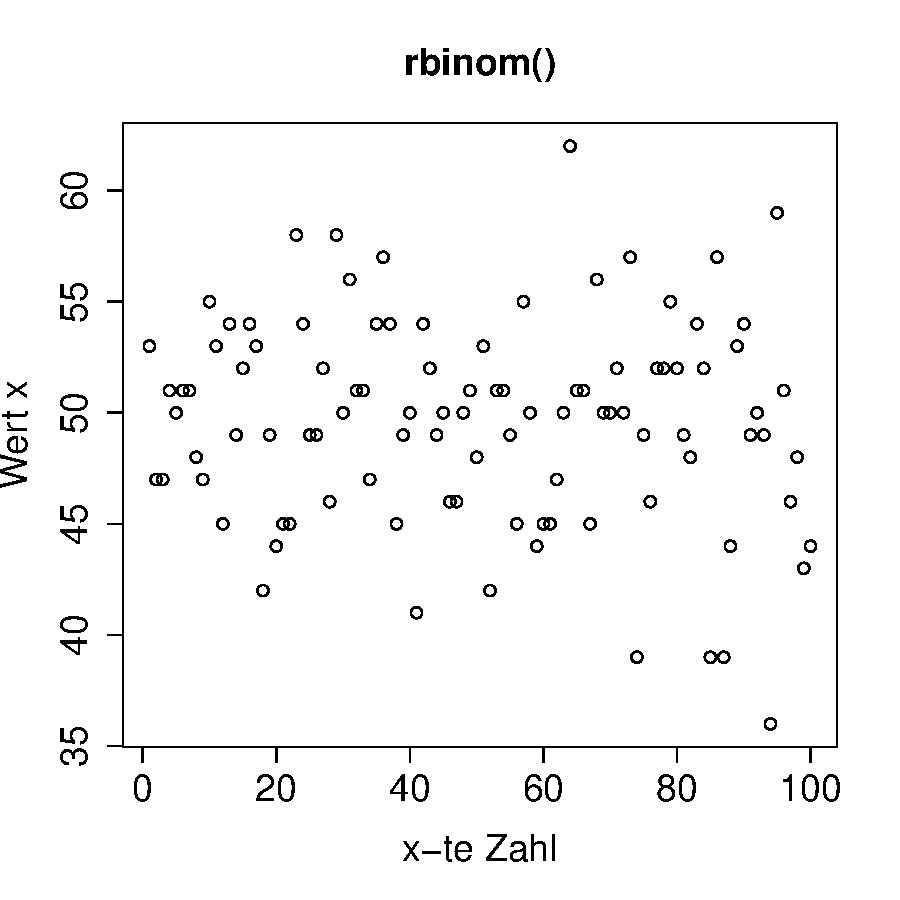
\includegraphics{verteilungen-021}
\caption{Zufallszahlen}
\end{subfigure}
\caption{Binomialverteilung ($n=100, p=0.5$)}
\label{fig:binom}
\end{figure}

\clearpage

\subsection{Beispiel einer binomialen Verteilung}
Jemand sagt Ihnen, dass er von 100 Münzwürfen 80 mal Kopf erhielt.
Sie antworten spontan, dass Sie ihm 15 Treffer von 20 Versuchen ja 
noch geglaubt hätten aber nicht 80 von 100. 
Wie wahrscheinlich sind aber diese beiden Ergebnisse wenn Kopf 
und Zahl jeweils gleichwahrscheinliche Ergebnisse sind?

\begin{Schunk}
\begin{Sinput}
> plot(dbinom(x=c(1:100), size=100, prob=0.5), type='h')
> plot(dbinom(x=c(1:20), size=20, prob=0.5), type='h')
\end{Sinput}
\end{Schunk}


\begin{figure}[h!]
\centering
\begin{subfigure}[b]{0.48\textwidth}
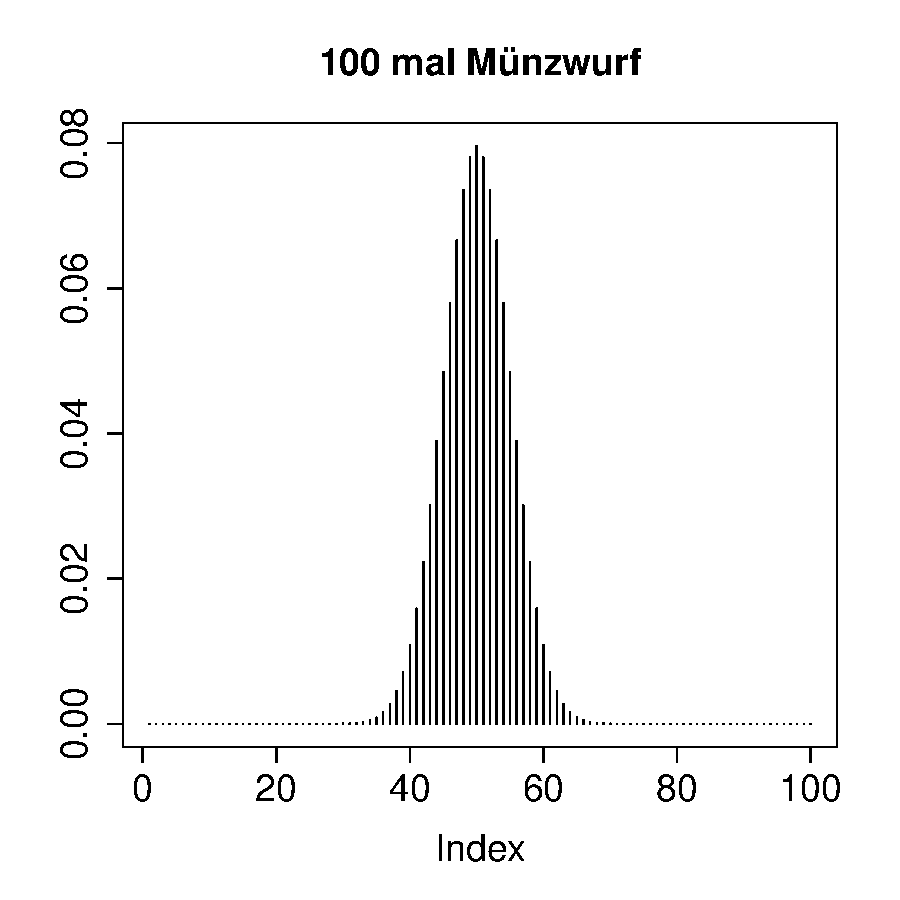
\includegraphics{verteilungen-025}
\caption{Verteilung für 100 Versuche}
\end{subfigure}
\begin{subfigure}[b]{0.48\textwidth}
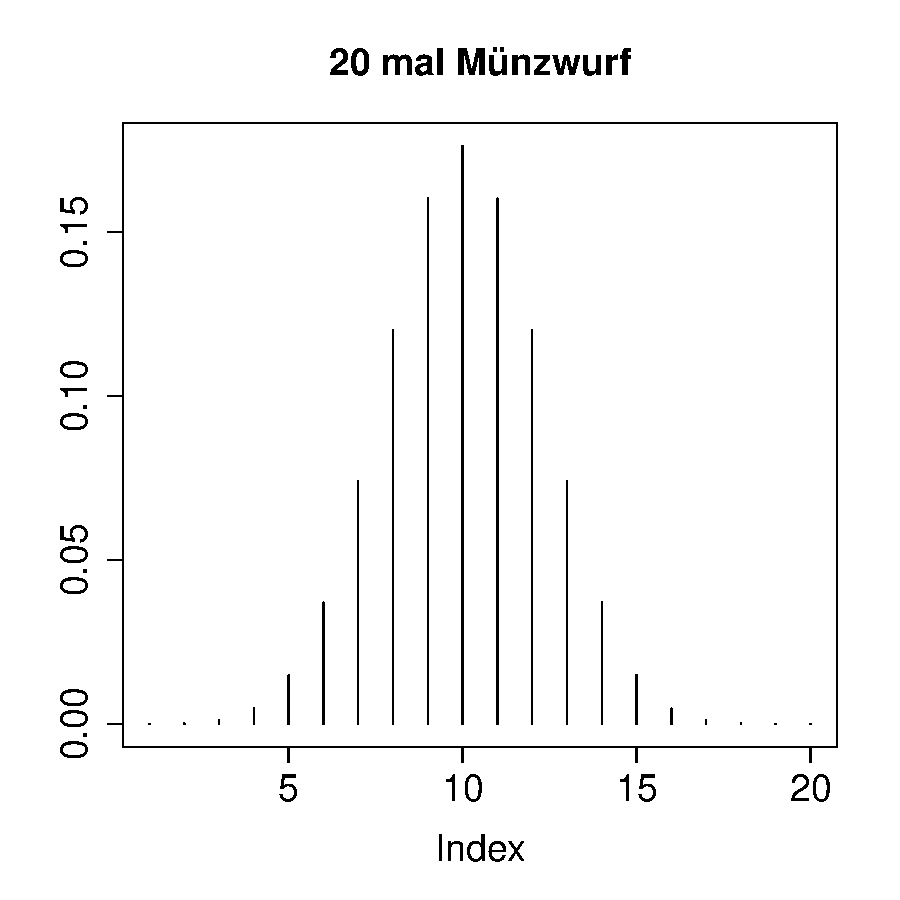
\includegraphics{verteilungen-026}
\caption{Verteilung für 20 Versuche}
\end{subfigure}
\caption{Wahrscheinlichkeitsverteilung beim Münzwurf}
\end{figure}

\clearpage
\newpage
\section{Poissonverteilung}
Die Poissonverteilung ist eine Verteilung welche Ereignisse
innerhalb eines Intervalls beschreibt. Dieses Intervall kann
eine beliebige skalare Grösse beschreiben wie Zeit, Länge oder
Temperatur \parencite[307]{oreilly}.

Die Poissonverteilung ist ein Spezialfall der Binomialverteilung
wenn die Anzahl Versuche $n$ gross und die 
Trefferwahrscheinlichkeit $p$ klein wird. Der Parameter $\lambda$
der Poissonverteilung ist definiert durch die Parameter einer
Binomialverteilung \parencite[197]{henze}.
\[ 
	\lambda := n \cdot p_n, \qquad Bin(n, p_n),\,n\geq1
\]
\[ 
	Bin(n,p) \xrightarrow{
		(n \rightarrow \infty) 
		\land
		(p \rightarrow 0)}
	Pois(\lambda)
\]

\noindent
Die Poissonverteilung beschreibt somit die Auftretenshäufigkeit 
innerhalb eines Intervalls. Der Parameter $\lambda$ beschreibt
sowohl den Erwartungswert als auch die Steuung. Dies definiert
das spezielle Verhalten dieser Verteilung, denn je höher der
Wert von $\lambda$ ist, desto flacher wird die Verteilung 
(siehe Abbildung \ref{fig:poisfall}).



\begin{figure}[h!]
\centering
\begin{subfigure}[b]{0.48\textwidth}
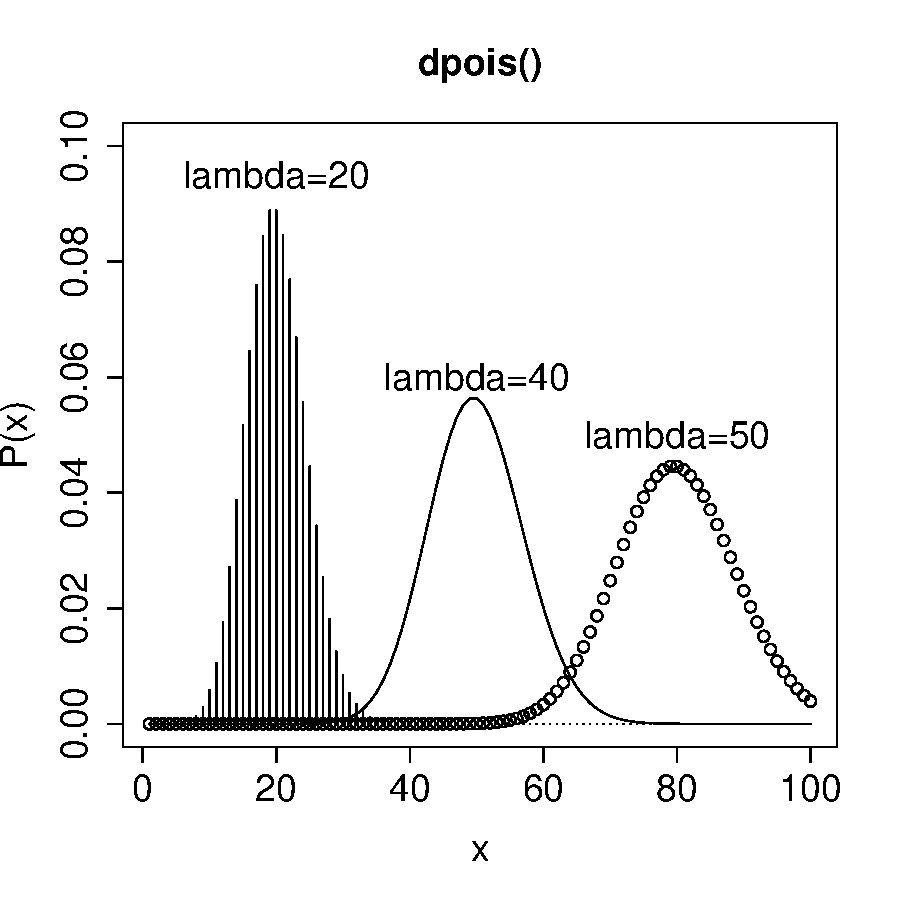
\includegraphics{verteilungen-028}
\end{subfigure}
\caption{Poissonverteilung für verschiedene $\lambda$}
\label{fig:poisfall}
\end{figure}

\newpage

\subsection{Verteilungsfunktion}
Die Verteilungsfunktion der Poissonverteilung ist definiert
durch den Erwartungswert $\lambda$ und die Anzahl der eintretenden
Ereignisse $x$.
\[  
	X \sim Pois(\lambda)
\]
\[  \begin{array}{l l}
	\lambda	
		& \text{Erwartungswert}
\end{array} \]
\[  
	P(X=x) = e^{-\lambda} \cdot \frac{\lambda^x}{x!}
\]

\subsection{Addition}
Mit dem Additionsgesetz für stochastisch unabhängige Zufallsvariablen 
können auch poissonverteilte Zufallsvariablen zusammengefasst werden.
\[  
	\left.\begin{array}{l l}
		X \sim Pois(\mu_1) & \\
		& \\
		Y \sim Pois(\mu_2) & \\
	\end{array} \right\} 
	\Rightarrow (X+Y) \sim Pois(\mu_1 + \mu_2)
\]

\subsection{Erwartungswert}
Der Erwartungswert der Poissonverteilung ist direkt ein Parameter
der Verteilungsfunktion selbst, nämlich $\lambda$.
\[  
	E(X) = \lambda = Var(X) 
\]

\subsection{Varianz}
Die Varianz einer Poissonverteilung ist wie der Erwartungswert durch den 
Parameter $\lambda$ der Verteilungsfunktion gegeben.
\[  
	Var(X) = \lambda = E(X)
\]

\subsection{Verwendung in R}
\lstinline{R} stellt grundsätzlich vier Funktionen für die 
Poissonverteilung zur Verfügung. 
\begin{itemize}
	\item \lstinline{dpois()} \hfill{} 
		(\emph{Wahrscheinlichkeitsverteilung})
	\item \lstinline{pois()} \hfill{}
		(\emph{kumulative Wahrscheinlichkeit})
	\item \lstinline{qpois()} \hfill{}
		(\emph{Verteilung der Quantile})
	\item \lstinline{rpois()} \hfill{}
		(\emph{Zufallszahlen})
\end{itemize}





\begin{figure}[h!]
\centering
\begin{subfigure}[b]{0.48\textwidth}
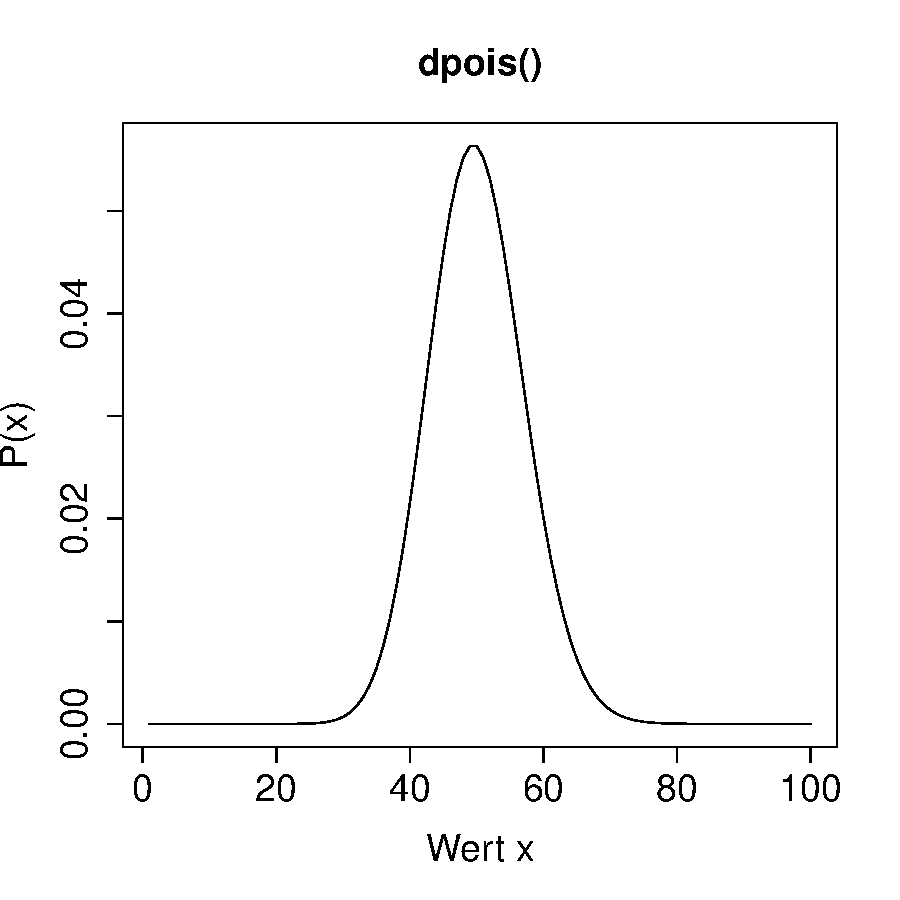
\includegraphics{verteilungen-033}
\caption{Wahrscheinlichkeitsverteilung}
\end{subfigure}
\begin{subfigure}[b]{0.48\textwidth}
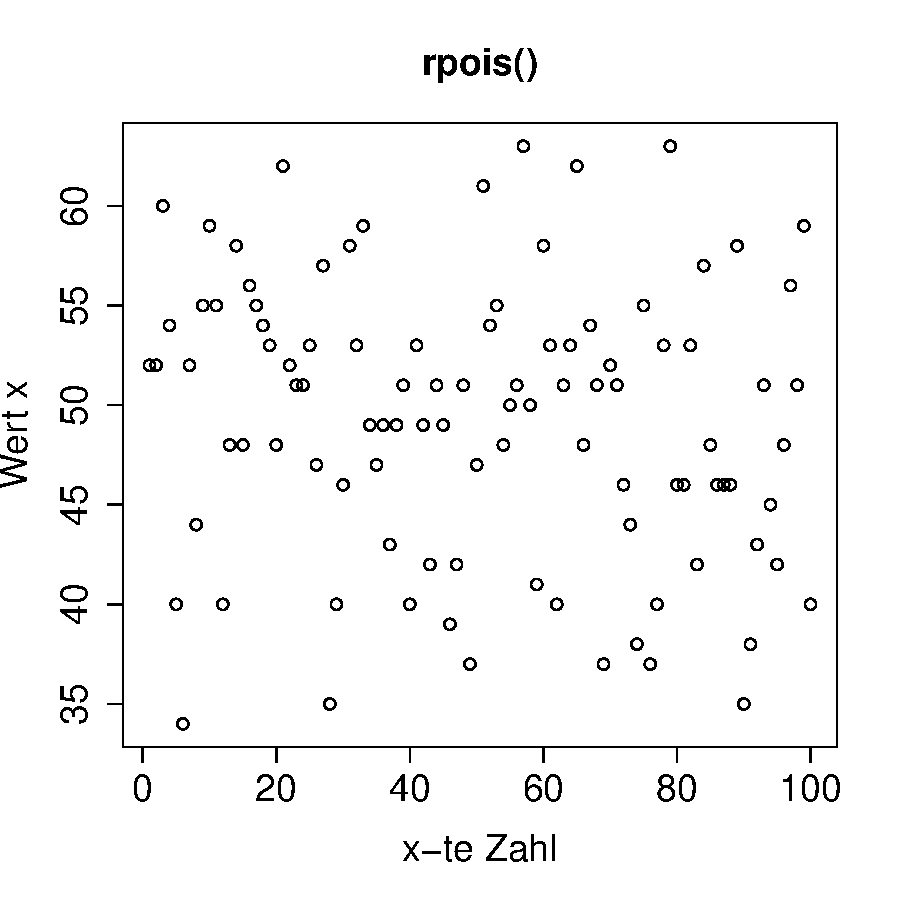
\includegraphics{verteilungen-034}
\caption{kumulative Wahrscheinlichkeit}
\end{subfigure}

\begin{subfigure}[b]{0.48\textwidth}
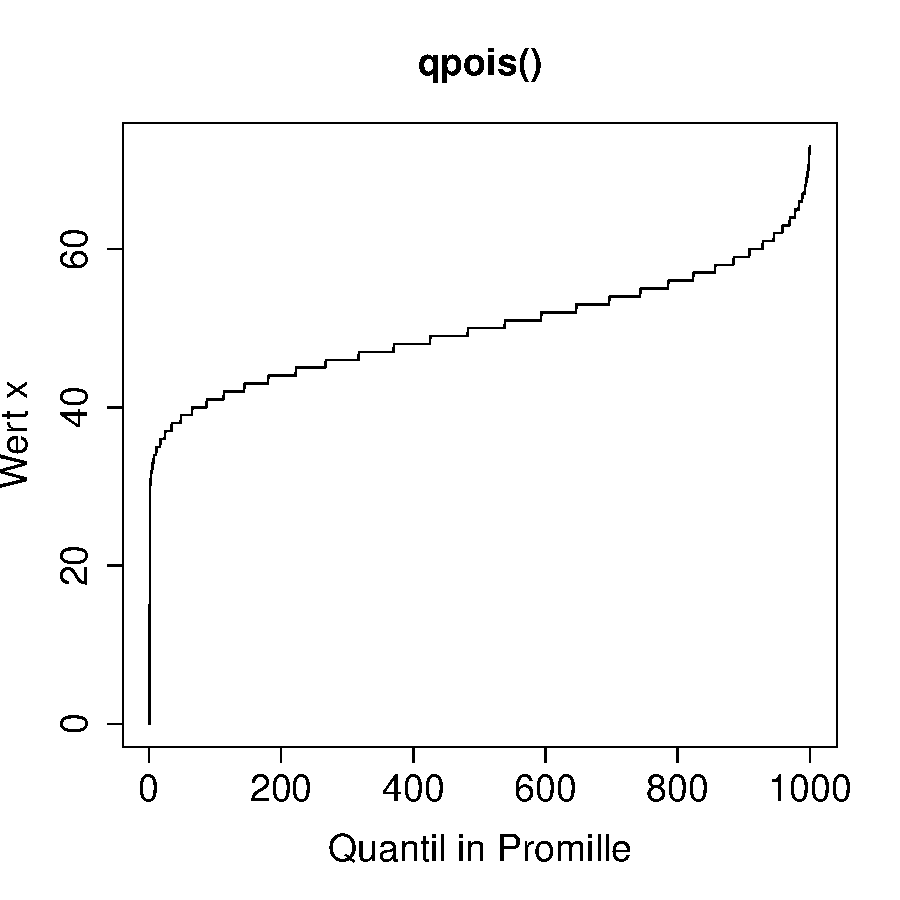
\includegraphics{verteilungen-035}
\caption{Quantile}
\end{subfigure}
\begin{subfigure}[b]{0.48\textwidth}
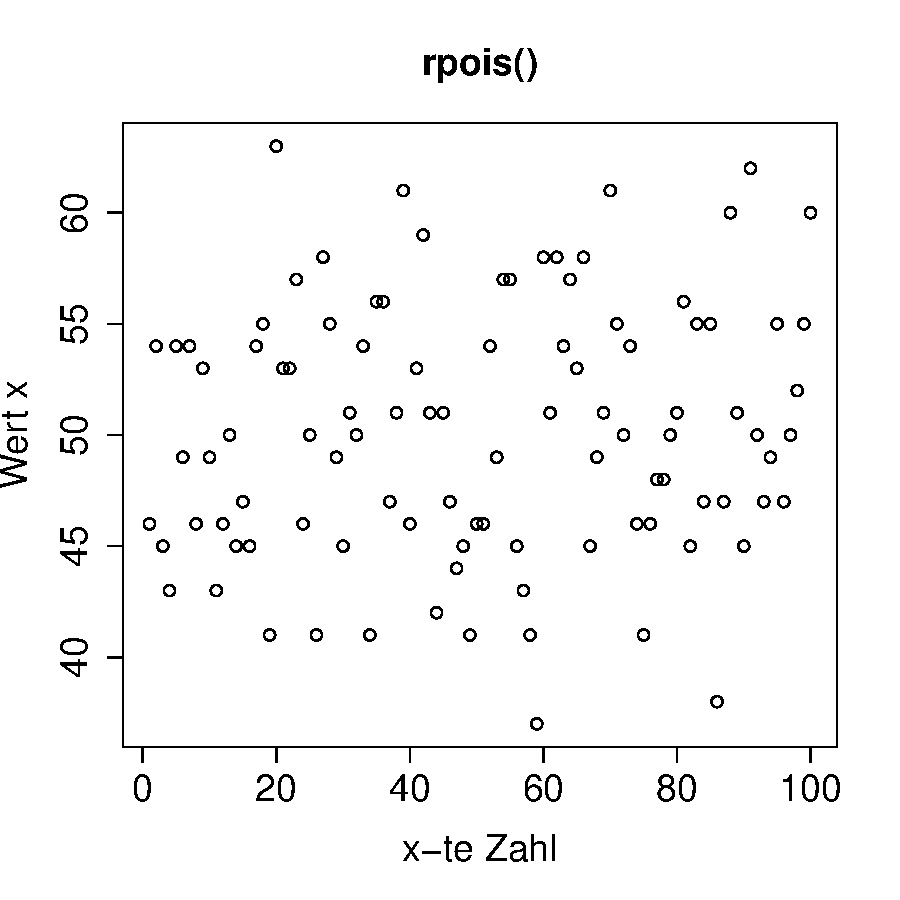
\includegraphics{verteilungen-036}
\caption{Zufallszahlen}
\end{subfigure}
\caption{Poissonverteilung ($\lambda=50$)}
\end{figure}

\clearpage

\subsection{Beispiel einer Poissonverteilung}

\paragraph{Beispiel 1 - Pixelfehler}
Ein \gls{Mikrocontroller} steuert ein Display an mit 320x240 
\gls{Pixel}. Damit möglichst schnelle Bildfolgen erzielt werden, 
haben sich die Programmierer bis an die Grenzen der Senderate und 
leicht darüber bewegt. Sie stellen nämlich fest, dass im Schnitt 
pro Bild (320x240 Pixel) ca. 12 Pixelfehler vorkommen.

Die Programmierer besprechen die Lage und einer meint: 
"`\emph{Rechnen wir doch mal die Wahrscheinlichkeit für höchstens 
einen Fehler aus und für mindestens 16, was unsere Schmerzgrenze 
sein soll.}"'

\begin{Schunk}
\begin{Sinput}
> eps <- 12 # error per screen
> # probability of at most 1 error per screen
> ppois(q=1, lambda=eps)
\end{Sinput}
\begin{Soutput}
[1] 7.987476e-05
\end{Soutput}
\begin{Sinput}
> # probability of at least 16 errors per screen
> 1-ppois(q=(16-1), lambda=eps)
\end{Sinput}
\begin{Soutput}
[1] 0.1555843
\end{Soutput}
\end{Schunk}



\begin{figure}[h!]
\centering
\begin{subfigure}[b]{0.48\textwidth}
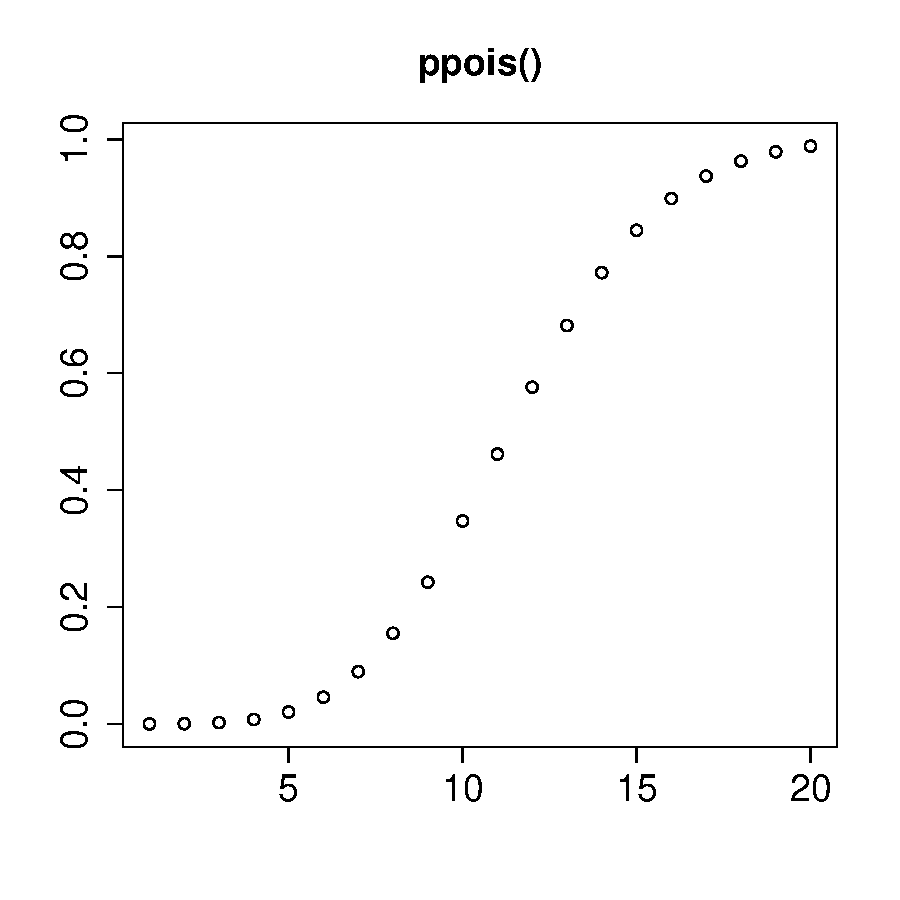
\includegraphics{verteilungen-040}
\caption{Punktwahrscheinlichkeit}
\end{subfigure}
\begin{subfigure}[b]{0.48\textwidth}
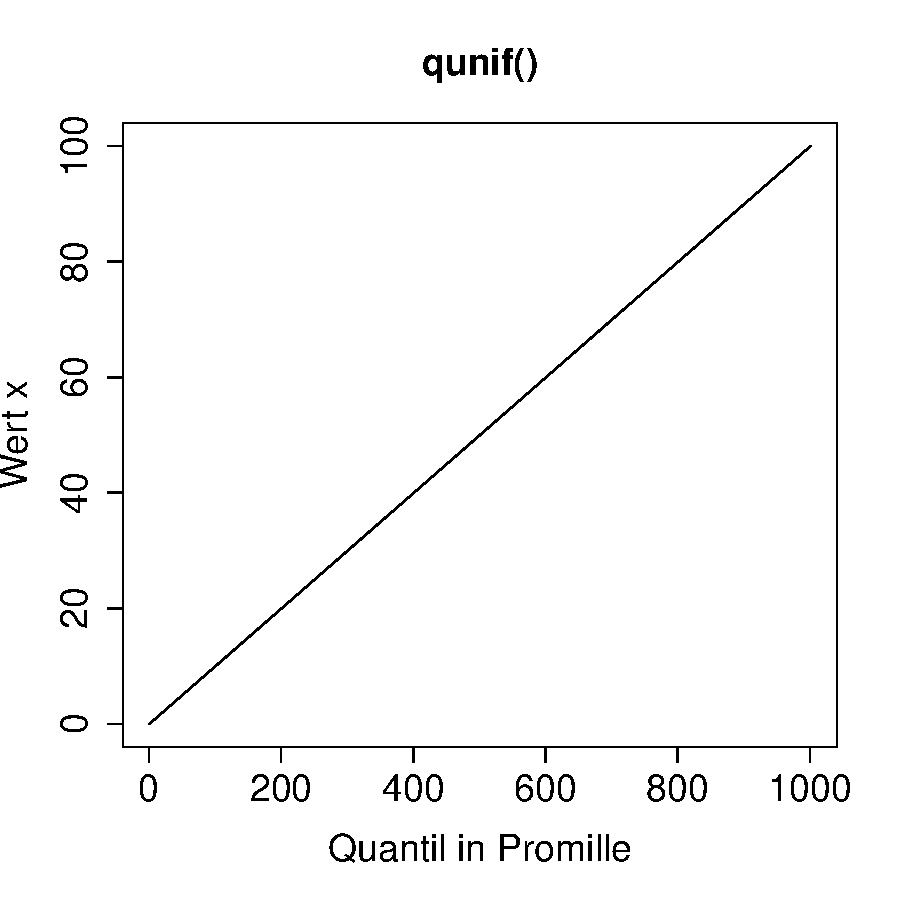
\includegraphics{verteilungen-041}
\caption{$1-$kummulative Wahrsch.}
\end{subfigure}
\caption{Wahrscheinlichkeiten von Pixelfehlern pro Bild}
\label{fig:embedded}
\end{figure}

\paragraph{Beispiel 2 --- Requests pro Woche}
Ein Team hat ein \gls{Embedded System} entwickelt, welches
Solarbetrieben an einem entlegenem Ort Geodaten sammelt und diese
über einen auf dem Embedded System implementierten Webserver
zur Verfügung stellt. Jedes Wochenende geht eine Gruppe von 
Studenten hin und prüft das System, macht Resets und flasht Updates.

Das Entwicklerteam erfährt am Montagmorgen, dass im letzten Update
ein Bug drin ist. Dieser verursacht nach einer gewissen Anzahl
an Requests einen \gls{Buffer Overflow}, welcher das System 
zum Absturz bringt. Die Entwickler schätzen, dass schon nach ca. 15 
Requests das dedizierte Embedded System abstürzen sollte.

Nun müssen die Entwickler sich entscheiden ob sie bis zum nächsten
Wochenende abwarten können um dem Bugfix zu flashen oder ob sie
noch vor dem Wochenende losziehen müssen. Sie sehen sich die alten
Logfiles an und bemerken, dass im Schnitt ca. zwei der kritischen
Requests pro Tag stattfinden.

Die Entwickler kennen mit diesen Informationen alles was sie
brauchen um die Frage korrekt aufzustellen: "`\emph{Wie gross
ist die Wahrscheinlichkeit, dass bis zum Wochenende mehr als 
15 Requests eintreffen?}"'

\begin{Schunk}
\begin{Sinput}
> hpd <- 2 # hits per day
> hpw <- hpd*7 # hits per week
> # probability of at least 15 hits in one week
> 1-ppois(q=(15-1), lambda=hpw)
\end{Sinput}
\begin{Soutput}
[1] 0.4295633
\end{Soutput}
\end{Schunk}



Die Analyse mit \lstinline{R} hat ergeben, dass die 
Wahrscheinlichkeit von mindestens 15 Requests bei ca. $0.43$ liegt
($1-$kummulative Verteilung, siehe Plot aus Abbildung \ref{fig:embedded}).

Die Entwickler lehnen sich also vorerst mal zurück mit dem Argument,
dass die Wahrscheinlichkeit von mehr als 15 Request bis zum 
Wochenende weniger als $50\%$ beträgt. Das seien ja schlechtere Chancen
als bein Münzwurf\dots


\begin{figure}[h!]
\centering
\begin{subfigure}[b]{0.48\textwidth}
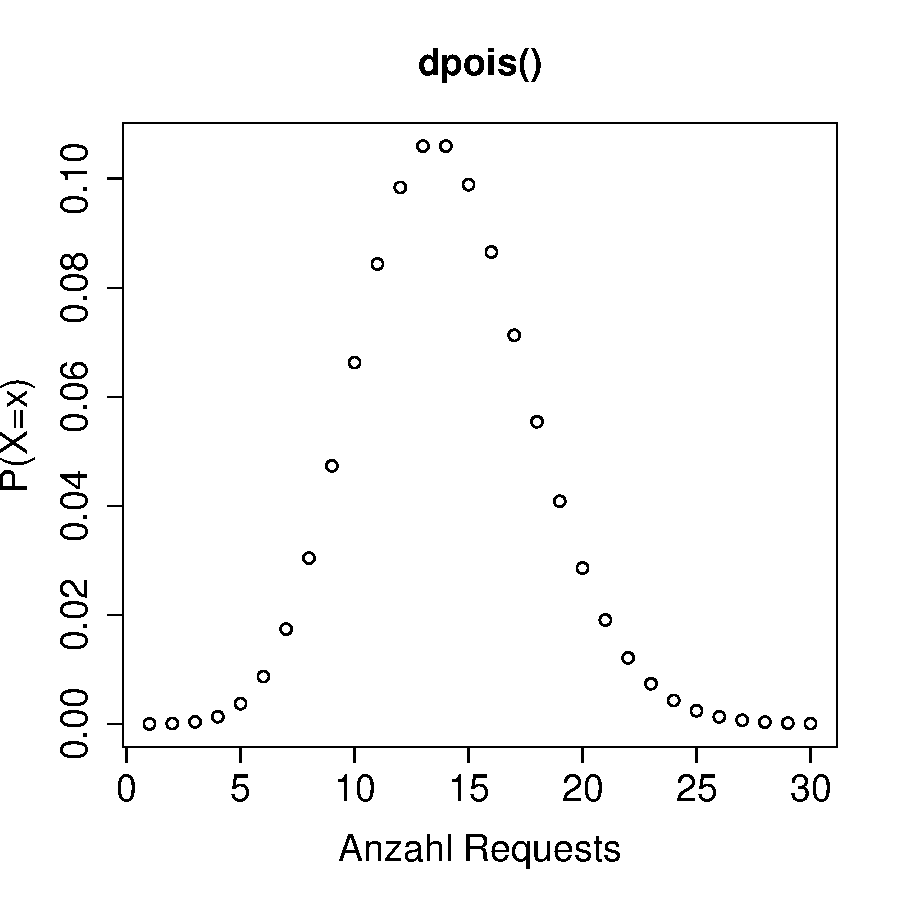
\includegraphics{verteilungen-046}
\caption{Punktwahrscheinlichkeit}
\end{subfigure}
\begin{subfigure}[b]{0.48\textwidth}
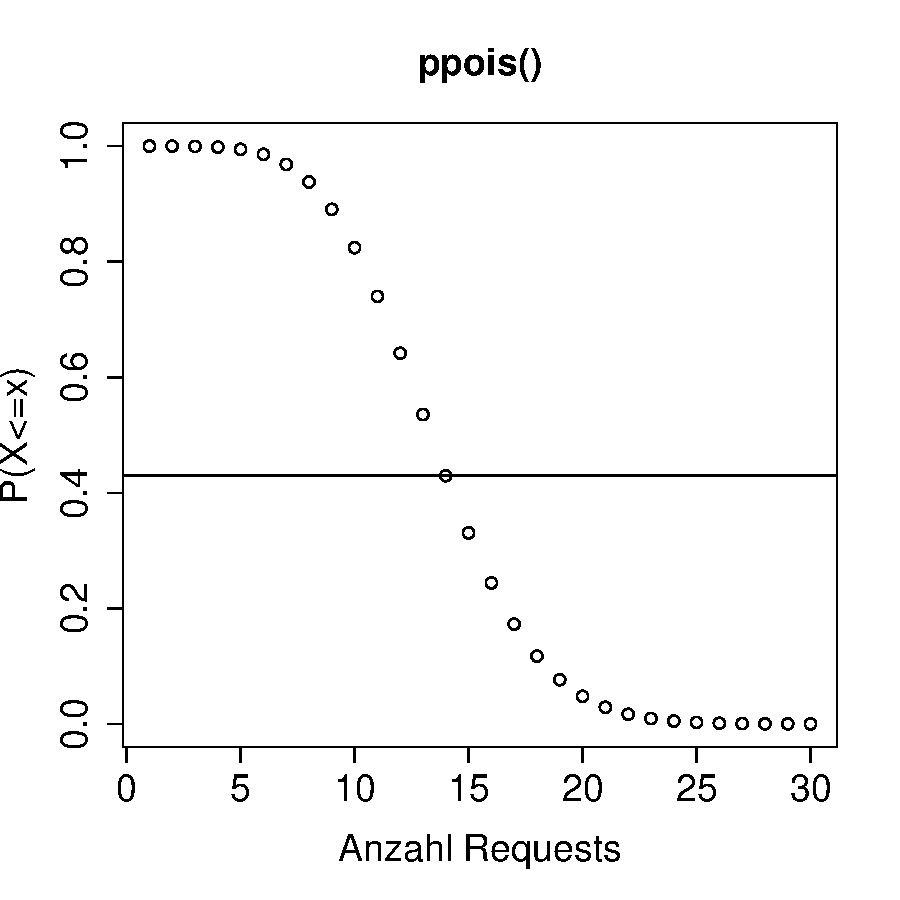
\includegraphics{verteilungen-047}
\caption{$1-$kummulative Wahrsch.}
\end{subfigure}
\caption{Wahrscheinlichkeiten von Requests pro Woche}
\label{fig:embedded}
\end{figure}


\clearpage

\section{Erwartungswert}
Der Erwartungswert einer diskreten Verteilung gibt jene Zahl an,
welche die Zufallsvariable im \emph{Mittel} annimmt. Sie beschreibt
quasi den mittleren Wert der Verteilung.

Für diskrete Wahrscheinlichkeitsverteilungen gilt, dass der 
Erwartungswert der Summe von Produkten aus Wahrscheinlichkeit und
Wert der Zufallsvariable entspricht. 
\[ \mu = E(X) = \sum x \cdot P(X=x) \]
$P(X=x)$ bedeutet \emph{Wahrscheinlichkeit, dass die Zufallsvariable $X$ 
genau $x$ ist}.

\subsection{Additivität von Erwartungswerten}
Erwartungswerte stochastisch unabhängiger Zufallsvariablen lassen sich
addieren
\[  
	E(X_1 + X_2) = E(X_1) + E(X_2)
\]
als auch subtrahieren
\[  
	E(X_1 - X_2) = E(X_1) - E(X_2)
\]

\section{Varianz}
Die Varianz einer Wahrscheinlichkeitsverteilung gibt ein Mass an für 
die Streuung der Warscheinlichkeiten um den Erwartungswert.

Die Varianz wird analog zum Erwartungswert ermittelt, wobei der Wert
der Zufallsvariable $x$ ersetzt wird durch das Quadrat der Abweichung
von Zufallsvariable und Erwartungswert $(x-\mu)^2$
\[ \begin{array}{l c l}
	Var(X) 
		& = 
		& E(X-\mu)^2 \\
	& &  \\
	Var(X)
		& = 
		& \sum \left( (x-\mu)^2 \cdot P(X=x) \right)
\end{array} \]

\subsection{Additivität von Varianzen}
Ähnlich wie Erwartungswerte lassen sich auch Varianzen addieren
\[  
	Var(X_1 + X_2) = Var(X_1) + Var(X_2)
\]
und auch subtrahieren. Bei der Subtraktion gilt es zu beachten,
dass die eigentliche Rechnung, eine Addition darstellt
\parencite[231]{oreilly}.
\[  
	Var(X_1 - X_2) = Var(X_1) + Var(X_2)
\]

\section{Lineare Transformation}
Die lineare Transformation beschreibt die lineare Änderung
der Verteilung einer Zufallsvariablen, wobei die Verteilung
im eigentlichen Sinne beibehalten wird, jedoch Erwartungswert
und Varianz sich verändern. Die Transformation wird linear
genannt, wenn die Änderung mittels eines Polynoms vom 
Grad 1 beschrieben wird.
\[  
	Y = a \cdot X + b
\]
Begrifflich kann die oben gezeigte lineare Transformation weiter
unterteilt werden in 
\begin{itemize}
	\item Nullpunkttransformation \hfill{} ($+b$)
	\item Einheitentransformation \hfill{} ($a \cdot X$)
\end{itemize}

Die lineare Transformation kann direkt auf den Erwartungswert
und die Varianz übertragen werden.
\[  
	E(Y) = E(a \cdot X + b) = a \cdot E(X) + b
\]
Bei der Transformation der Varianz gilt es zu beachten, dass
die Nullpunkttransformation hinfällig ist und die
Einheitentransformation quadratisch wirkt.
\[  
	Var(Y) = Var(a \cdot X +b) = a^2 \cdot Var(X)
\]
Der mathematische Hintergrund für diese Berechnung der Varianz
liegt in der sog. \emph{linearität des Integrals}, welche im 
eigentlichen besagt, dass konstante Faktoren vor das Integral
genommen werden können und Summen separierbar sind.

Einfacher ist allerdings die graphische Erklärung. Die Abbildung
\ref{fig:lintrans} zeigt auf, dass die Multiplikation mit $a$ 
sich auf die Steuung auswirkt, nicht aber die Addition von $b$. 
Wenn alle Punkte um den selben Wert in die selbe Richtung 
verschoben werden, so ändert dies nicht deren Steuung.



\begin{figure}[h!]
\centering
\begin{subfigure}[b]{0.48\textwidth}
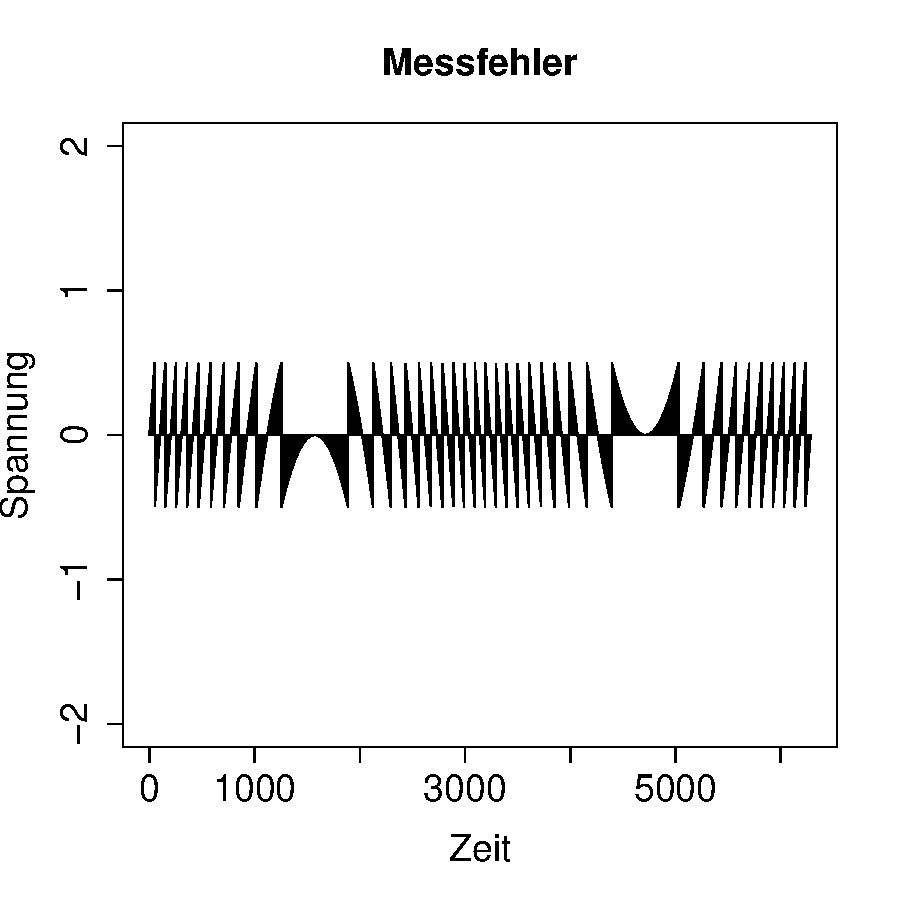
\includegraphics{verteilungen-050}
\caption{Zufallsvariable $X$}
\end{subfigure}
\begin{subfigure}[b]{0.48\textwidth}
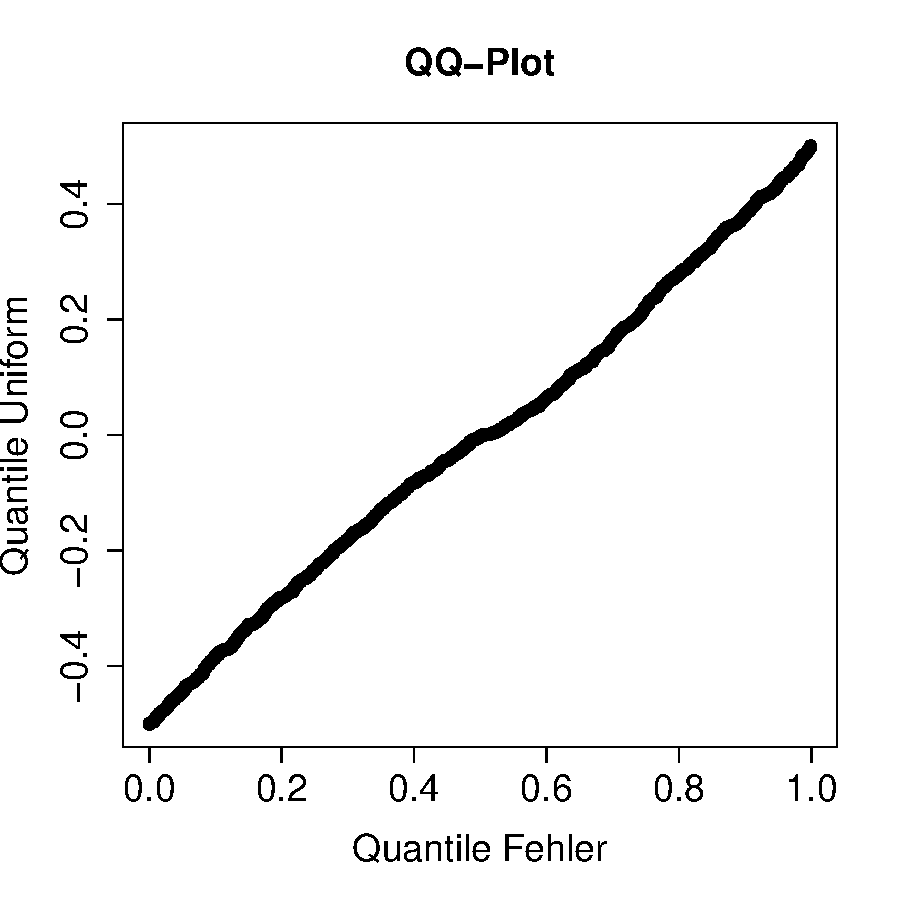
\includegraphics{verteilungen-051}
\caption{Zufallsvariable $Y=3\cdot X +2$}
\end{subfigure}

\rule[1mm]{0mm}{5mm}

\begin{subfigure}[b]{1\textwidth}
\centering
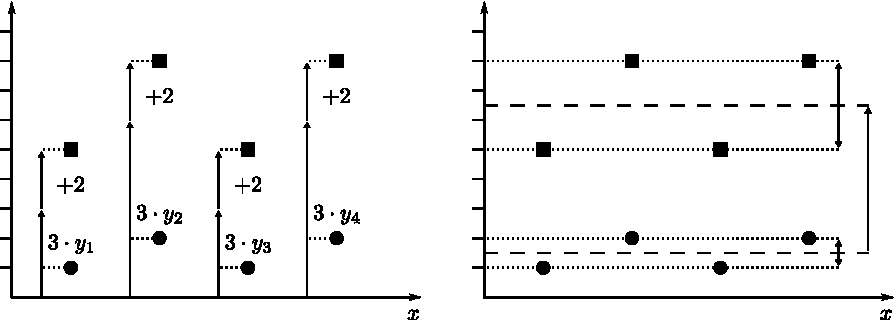
\includegraphics[width=0.9\textwidth]{lintrans.pdf}
\caption{Graphische Analyse der Transformation}
\end{subfigure}

\caption{Lineare Transformation $Y = 3 \cdot X + 2$}
\label{fig:lintrans}
\end{figure}

\section{Standardabweichung}
Die Standardabweichung einer Wahrscheinlichkeitsverteilung 
ist wie die Varianz ein Mass für die Streuung. Sie 
wird anhand der Varianz ermittelt mit dem Zusammenhang, dass die 
Standardabweichung der Quadratwurzel der Varianz entspricht.
\[ \begin{array}{l c l} 
	\sigma 
		& = 
		& \sqrt{Var(X)} \\
	& & \\
	\sigma
		& =
		& \sqrt{E(X-\mu)^2} \\
	& & \\
	\sigma
		& =
		& \sqrt{\sum \left( (x-\mu)^2 \cdot P(X=x) \right)}
\end{array} \]

\section{Zusammenfassung}
Diskrete Verteilungen kommen bei Problemen vor die immer Ergebnisse
aus $\mathbb{N}$ liefern. Von diesen gibt es drei elementare Verteilungen.

\begin{itemize}
	\item Hypergeometrische Verteilung 
		\hfill{} (\emph{Ziehen ohne Zurücklegen})
	\item Binomialverteilung 
		\hfill{} (\emph{Münzwurf})
	\item Poissonverteilung 
		\hfill{} (\emph{nach oben offen})
\end{itemize}

\noindent
Diese drei Verteilung stehen in einem engen Verhältnis, denn die
Binomialverteilung ist ein Spezialfall der Hypergeometrischen 
Verteilung und die Poissonverteilung ist ein Spezialfall der
Binomialverteilung. Dies zeigt sich in der Reduktion der Parameter.
\[ \begin{array}{c c c c c}
	Hyp(n,r,s)
		& \xrightarrow{n,s \rightarrow \infty}
		& Bin(n,p)
		& \xrightarrow{n,p_n \rightarrow \lambda}
		& Pois(\lambda) \\
	3 \text{ Parameter}
		& 
		& 2 \text{ Parameter}
		& 
		& 1 \text{ Parameter}
\end{array} \]

\noindent
Um jeweils die richtige Verteilung zu wählen, kann man folgende Merkregeln 
beachten.

\begin{description}
	\item[Hypergeometrisch]
		Jedes Ereignis (Treffer oder Niete) verändert den 
		Grundraum.
	\item[Binomial] Jedes Ereignis hat die gleiche 
		Wahrscheinlichkeit. Diese Verteilung ist zu wählen,
		wenn man wissen möchte, wie viele Treffer für eine
		bestimmte Anzahl Versuche eintreten.
	\item[Poisson] Man hat eine Erwartung von der Anzahl 
		eintretender Ereignisse (Treffer) und möchte wissen,
		wie viele Treffer in einem bestimmten Intervall 
		eintreten.
\end{description}

\subsection{Erwartungswert und Varianz}

\begin{table}[h!]
	\centering
	\begin{tabular}{l c c}
		Verteilung
			& $E(X)$
			& $Var(X)$ \\
		\hline
		& & \\
		$X \sim Hyp(n,r,s)$
			& $n \cdot \left(\frac{r}{N}\right)$
			& $n \cdot \left( 
				\frac{r}{N}
				\right) 
			\left( 
				1 - \frac{r}{N}
			\right)
			\left(
				\frac{(N)-n}{(N)-1}
			\right)$ \\
		& & \\
		$X \sim Bin(n,p)$
			& $n \cdot p$
			& $n \cdot p \cdot (1-p)$ \\
		& & \\
		$X \sim Pois(\lambda)$
			& $\lambda$
			& $\lambda$
	\end{tabular}
\end{table}

\subsection{Berechnungen in R}

\begin{table}[h!]
	\begin{tabular}{l l l}
	$X \sim Hyp(n,r,s)$ & & \\ %\hline
		& genau $A$ 		& \verb!dhyper(x=A,...)! \\
		& höchstens $A$		& \verb!phyper(q=A,...)! \\
		& mindestens $A$	& \verb!1-phyper(q=A-1,...)! \\
		& $A$ zufällige 	& \verb!rhyper(n=A...)! \\
	& & \\
	$X \sim Bin(n,p)$ & & \\ %\hline
		& genau $A$		& \verb!dbinom(x=A,...)! \\
		& höchstens $A$		& \verb!pbinom(q=A,...)! \\
		& mindestens $A$	& \verb!1-pbinom(q=A-1,...)! \\
		& $A$ zufällige 	& \verb!rbinom(n=A...)! \\
	& & \\
	$X \sim Pois(\lambda)$ & & \\ %\hline
		& genau $A$		& \verb!dpois(x=A,...)! \\
		& höchstens $A$		& \verb!ppois(q=A,...)! \\
		& mindestens $A$	& \verb!1-ppois(q=A-1,...)! \\
		& $A$ zufällige 	& \verb!rpois(n=A...)! \\
	\end{tabular}
\end{table}

\chapter{Stetige Verteilungen}
Stetige und absolut stetige Verteilungen beschreibebn Probleme, 
welche Ergebnisse aus $\mathbb{R}$ liefern.

\paragraph{Stetig} Die Eigenschaft der Stetigkeit ist so definiert,
dass die Punktwahrscheinlichkeit einer Zufallsvariable 
$X$ Null ergibt und $x$ auch wirklich jeden Wert aus
$\mathbb{R}$ annehmen kann.
\[ 
	P(X=x) = 0, \qquad x\in\mathbb{R}
\]
\paragraph{Absolute Stetigkeit}
Als absolut stetig werden Funktionen beschrieben die integrierbar 
sind. 

\newpage

\section{Dichtefunktion}
Die Dichtefunktion $f(x)$ ist definiert als die Ableitung der kummulativen
Verteilungsfunktion $F(x)$.
\[  
	\int f(x) := F(x) 
		\qquad 
		\Leftrightarrow 
		\qquad 
		f(x) = \frac{d}{dx} F(x)
		= F'(x)
\]
Mit der Dichte lässt sich eine Aussage darüber treffen, wie die 
Wahrscheinlichkeit ist, dass eine Zufallsvariable $X$ einen Wert
in einem bestimmten Intervall $[a,b]$ annimmt (siehe Grafik 
\ref{fig:dichte}).

\begin{figure}[h!]
	\centering
	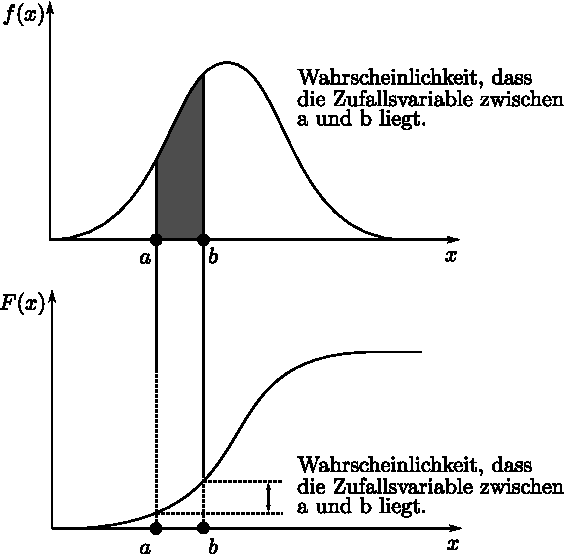
\includegraphics[width=0.7\textwidth]{dichtefunktion.pdf}
	\caption{Dichtefunktion $f(x)$ und kummulative Verteilungsfunktion 
		$F(x)$ in der Gegenüberstellung.}
	\label{fig:dichte}
\end{figure}

Mit der Definition der Dichtefunktion $f(x)$ lassen sich mehrere 
Gesetzmässigkeiten herleiten:
\begin{itemize}
	\item Die Dichte in einem Punkt $a$ ist Null.
		\[ f(x) = 0 
			\qquad \lim_{a_1 \rightarrow a_0} \left(
				\int_{a_0}^{a_1} f(x)\,dx \right) = 0   \]
	\item Das Integral einer Dichtefunktion über einem Intervall
		$[a,b]$ ist gleich der Differenz der kummulativen
		Wahrscheinlichkeiten von $a$ und $b$ (siehe Grafik 
		\ref{fig:dichte}).
		\[ \int_a^b f(X)\, dx = F(b) - F(a) \]
	\item Das Integral der Dichtefunktion über dem Intervall 
		$[-\infty, +\infty]$ ist genau 1 
		(siehe \gls{Axiome von Kolmogorov}, \gls{Normiertheit}).
		Dies bedeutet, dass die kummulative Verteilungsfunktion
		für grosse $x$ gegen $1$ strebt und für kleine gegen $0$.
		\[ \int_{-\infty}^{+\infty} f(x)\, dx = 1 \]
		\[ F(x) \xrightarrow{x \rightarrow +\infty} 1
			\qquad \Leftrightarrow \qquad 
			\lim_{x \rightarrow + \infty} 
				F(x) = 1 \]
		\[ F(x) \xrightarrow{x \rightarrow -\infty} 0 
			\qquad \Leftrightarrow \qquad
			\lim_{x \rightarrow - \infty} 
				F(x) = 0 \]
\end{itemize}

\subsection{Erwartungswert}
Der Erwartungswert einer stetigen Verteilung mit der Dichte $f(x)$ und 
der Funktion g(x) ist allgemein definiert als
\[ 
	E(g(X)) = \int_{-\infty}^{+\infty} g(x) \cdot f(x)\, dx
\]
Falls die Funktion $g(x)$ mit einer Variable gleichgesetzt werden
kann, also $g(x)=x$ gilt, dann kann der Erwartungswert auch berechnet
werden als
\[  
	E(X) = \int_{-\infty}^{+\infty} x \cdot f(x)\, dx,
		\qquad x = g(x)
\]

\subsection{Varianz}
\[ \begin{array}{l c l} 
	Var(X) 
		& = 
		& \displaystyle 
			\int_{-\infty}^{+\infty} 
			(x-E(X))^2 \cdot f(x)\, dx \\
		& & \\
		& = 
		& E(X-E(X))^2 \\
		& & \\
		& = 
		& E(X^2) - E(X)^2
\end{array} \]

\subsection{Standardabweichung}
Die Standardabweichung wird wie bei den diskreten Verteilungen 
duch die Wurzel aus der Varianz ermittelt.
\[  
	\sigma_x = \sqrt{Var(X)}
\]

\subsection{Quantile}
Ein Quantil $q(\alpha)$ markiert (in \%) die $x$-Stelle einer 
Dichtefunktion $f(x)$, bei welcher der angegebene Anteil $\alpha$
darunter liegt.
\[ 
	q(\alpha), 
		\qquad \alpha = 
		\{x \mid 0 < x < 1 \land x \in \mathbb{R}\}
\]
\[
	P(X \leq q(\alpha)) = \alpha
\]
\[ 
	F(q(\alpha)) = \alpha  
		\qquad \Leftrightarrow \qquad
		F^{-1}(\alpha) = q(\alpha)
\]

\begin{figure}[h!]
	\centering
	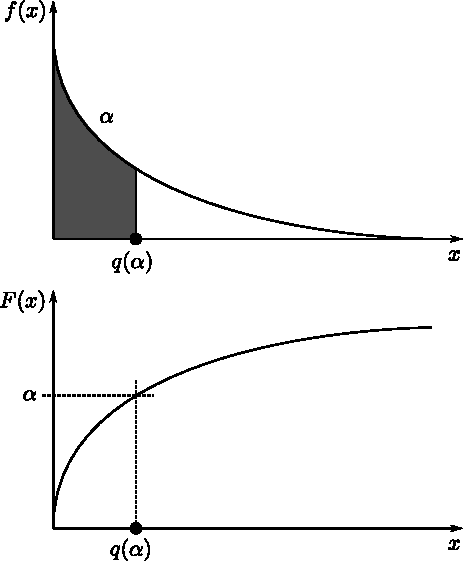
\includegraphics[width=0.7\textwidth]{dichtefunktion-quantile.pdf}
	\caption{Quantil einer Dichtefunktion.}
	\label{fig:dichte-quantil}
\end{figure}

\clearpage
\newpage
\section{Uniforme Verteilung}

Die uniforme Verteilung (auch \emph{Gleichverteilung}) ist eine
Verteilung, deren Wahrscheinlichkeit nur in einem bestimmten 
Intervall $[a,b]$ ungleich Null ist. Die Dichte $f(x)$ innerhalb 
des Intervalls $[a,b]$ ist konstant und ausserhalb davon gleich Null.
Zusammenfassend kann man sagen, dass die uniforme Verteilung eine
konstante Dichte hat.

\[  
	f(x) = \mathrm{konstant} = \left\{\begin{array}{c c l}
		\displaystyle \frac{1}{b-a}
			& \text{falls}
			& a < x < b \\
		& & \\
		0
			& \text{falls}
			& (x < a) \lor (x > b)
		\end{array} \right.
\]

\begin{figure}[h!]
	\centering
	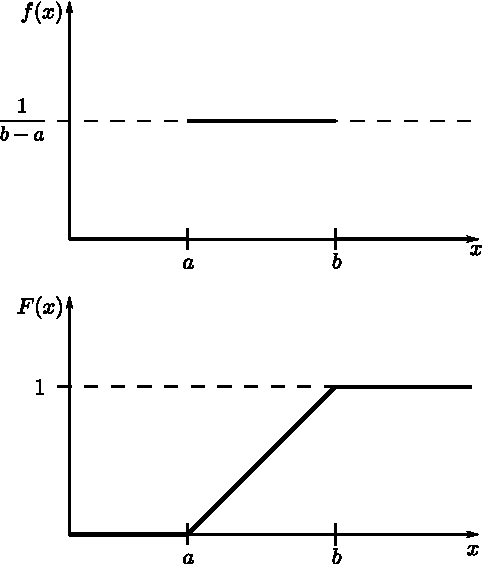
\includegraphics[width=0.7\textwidth]{uniform.pdf}
	\caption{Uniforme Dichte $f(x)$ und Verteilung $F(x)$.}
	\label{fig:uniform}
\end{figure}

\subsection{Verteilungsfunktion}
Die Verteilungsfunktion der uniformen Verteilung beschreibt
grundsätlich eine Gerade und wenn das Intervall 
$[a,b]\neq[-\infty, +\infty]$ ist, so ist diese Bereichsweise
definiert.

\[  
	F(x) = \left\{
		\begin{array}{c c l}
			0 
				& \text{falls } 
				& x < a \\
			& \\
			\displaystyle
			\frac{x-a}{b-a} 
				& \text{falls } 
				& a < x < b \\
			& \\
			1
				& \text{falls } 
				& b < x
		\end{array} \right.
\]

\subsection{Erwartungswert}
Da die Dichtefunktion der uniformen Verteilung konstant ist,
kann der Erwartungswert sehr einfach berechnet werden.
\[  
	E(X) = \frac{a+b}{2}
\]
Die Werte $a,b$ können auch als Minimal- bzw. Maximalwerte
betrachtet werden.
\[  
E(X) = \frac{\text{min} + \text{max}}{2}
\]

\subsection{Varianz}
Analog zum Erwartungswert ist auch die Berechnung der Varianz
einer uniformen Verteilung relativ einfach.
\[ 
	Var(X) = \frac{(b - a)^2}{12}
\]
Wie auch beim Erwartungswert, können die Intervallgrenzen
$[a,b]$ als Mininal- und Maximalwerte betrachtet werden.
\[  
	Var(X) = \frac{(\text{max} - \text{min})^2}{12}
\]

\subsection{Verwendung in R}
\lstinline{R} stellt grundsätzlich vier Funktionen für die 
uniforme Verteilung zur Verfügung. 
\begin{itemize}
	\item \lstinline{dunif()} \hfill{} 
		(\emph{Wahrscheinlichkeitsverteilung})
	\item \lstinline{punif()} \hfill{}
		(\emph{kumulative Wahrscheinlichkeit})
	\item \lstinline{qunif()} \hfill{}
		(\emph{Verteilung der Quantile})
	\item \lstinline{runif()} \hfill{}
		(\emph{Zufallszahlen})
\end{itemize}
Die Abbildung \ref{fig:unif} zeigt jeweils einen Plot zu den gegebenen
Funktionen aus \lstinline{R}. Für weitere Informationen zu Plots siehe
Kapitel \ref{sec:plots}.





\begin{figure}[h!]
\centering
\begin{subfigure}[b]{0.48\textwidth}
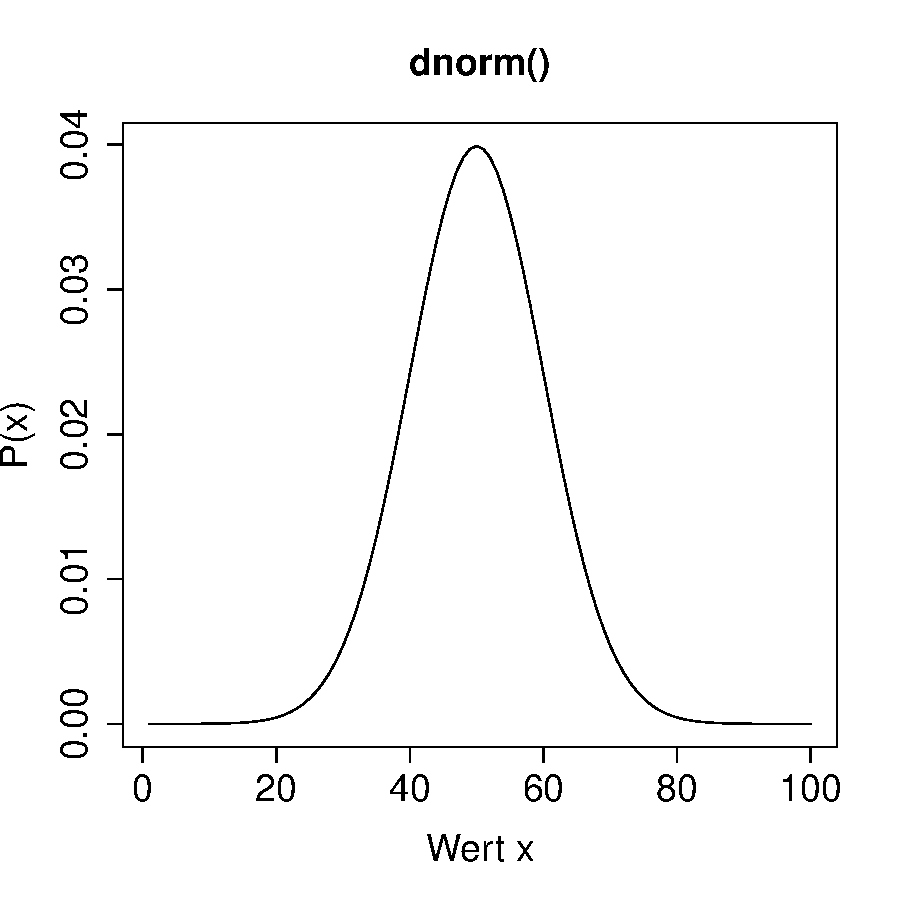
\includegraphics{verteilungen-056}
\caption{Wahrscheinlichkeitsverteilung}
\end{subfigure}
\begin{subfigure}[b]{0.48\textwidth}
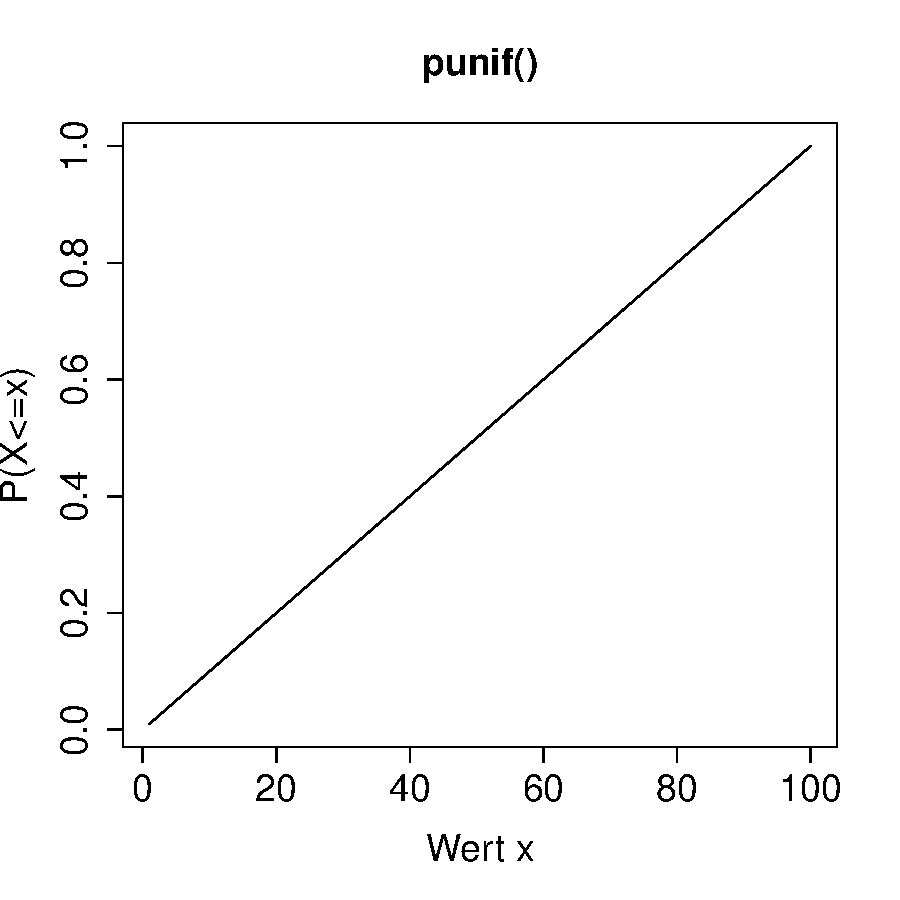
\includegraphics{verteilungen-057}
\caption{kumulative Wahrscheinlichkeit}
\end{subfigure}

\begin{subfigure}[b]{0.48\textwidth}
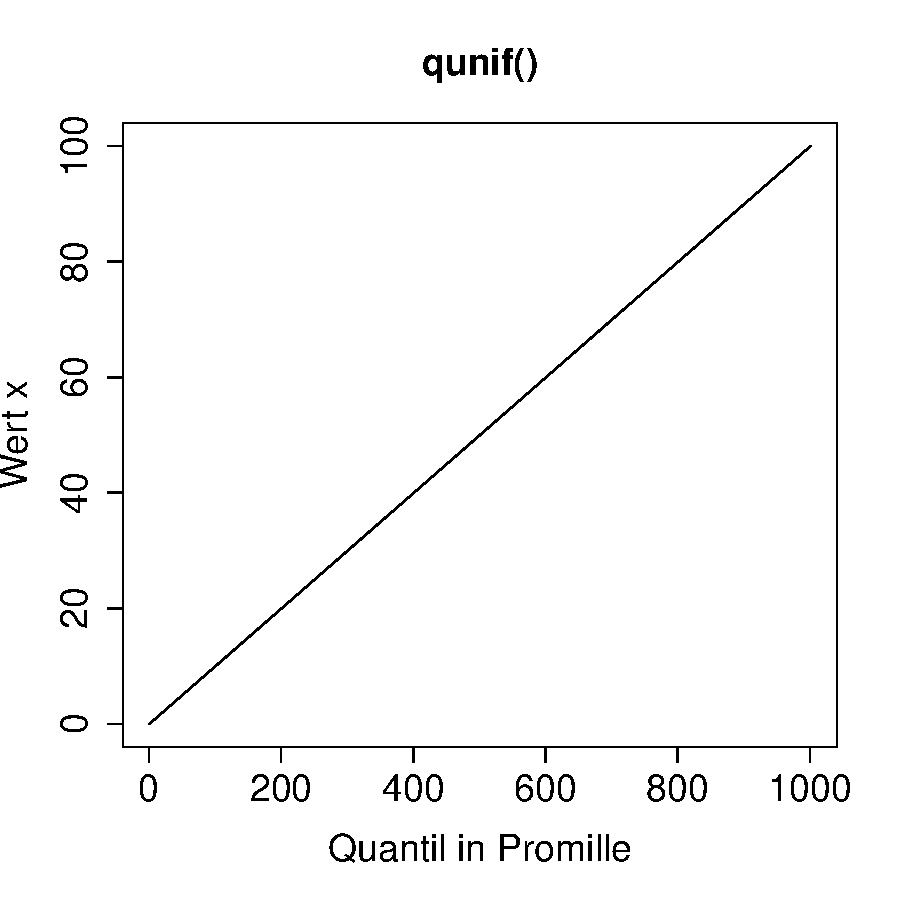
\includegraphics{verteilungen-058}
\caption{Quantile}
\end{subfigure}
\begin{subfigure}[b]{0.48\textwidth}
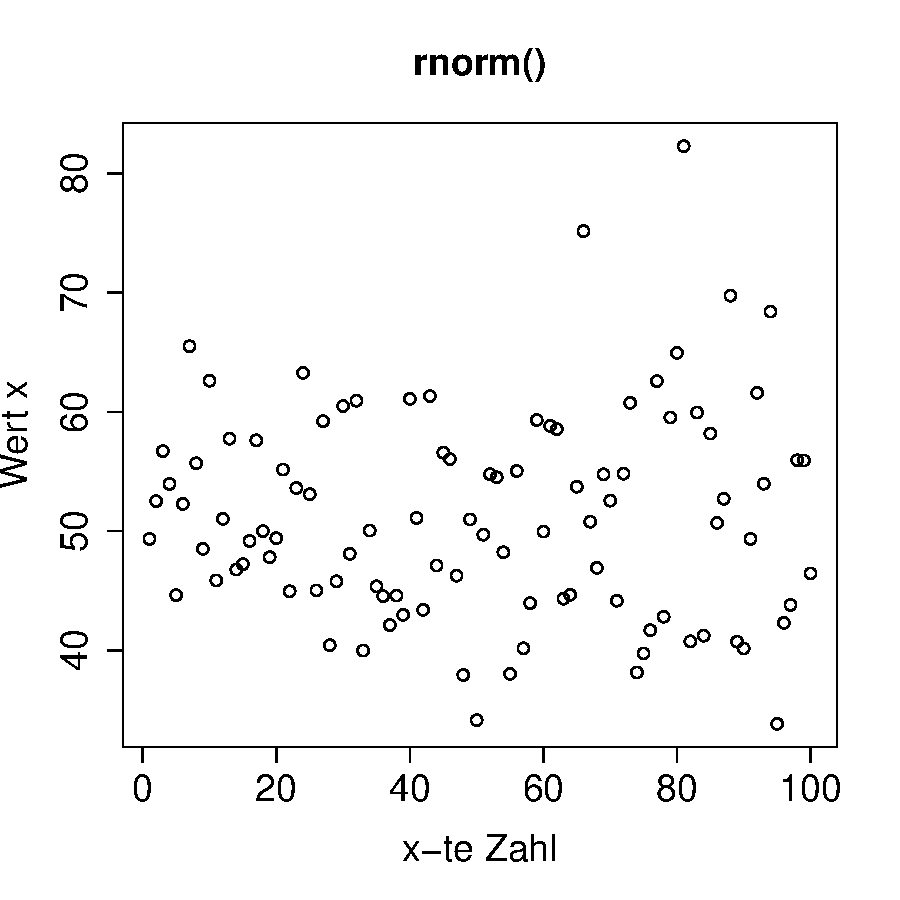
\includegraphics{verteilungen-059}
\caption{Zufallszahlen}
\end{subfigure}
\caption{Uniforme Verteilung ($n=100, min=0, max=100$)}
\label{fig:unif}
\end{figure}

\clearpage
\subsection{Beispiel einer uniformen Verteilung}
Benutzt man einen ADC (engl. \emph{Analog to Digital Converter}) zur 
Erfassung elektronischer Messgrössen als digitale Werte, so 
\emph{quantifziert} dieser die Messung und es entsteht ein Messfehler. 
Ist die zu erfassende Grösse viel grösser als die kleinstmögliche 
Auflösung des ADC, so ist dieser Fehler uniform verteilt 
\parencite[615]{taoe}. Typische Fehler beim Messverfahren werden oft
vom Hersteller für den jeweiligen ADC angegeben 
(siehe Anhang \ref{sec:stm32f21xx-adc}).

\begin{figure}[h!]
	\centering
	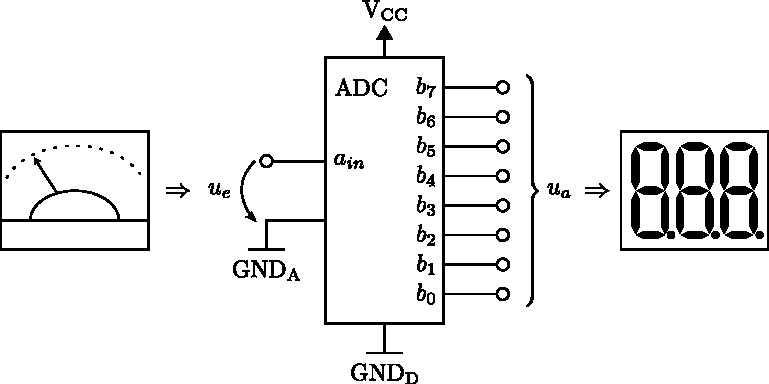
\includegraphics[width=0.95\textwidth]{adc-system.pdf}
	\caption{Analog-to-Digital Converter, 8 Bit.}
\end{figure}

\begin{Schunk}
\begin{Sinput}
> f1 <- 10*sin(x=seq(0, 2*pi, 0.001))
> adc.in  <- (f1)
> adc.out <- round(x=adc.in, digits=0)
> error   <- (adc.in - adc.out)
> m <-mean(error)
> s <-sd(error)
> m
\end{Sinput}
\begin{Soutput}
[1] -0.0001592544
\end{Soutput}
\begin{Sinput}
> s
\end{Sinput}
\begin{Soutput}
[1] 0.27766
\end{Soutput}
\end{Schunk}

\noindent
Mit Hilfe von R lässt sich dieses Beispiel relativ leicht rechnen und
plotten. Die Plots aus der Abbildung \ref{fig:adc} zeigen, dass die 
Quantifizireung des Eingangsignals einen uniformen Fehler verusrsacht.
Die Grafik \ref{fig:adc-d} zeigt den Beweis für die uniforme Verteilung
anhand eines Quantilenvergleichs mit einer ideal uniform verteilten
Datenreihe.





\begin{figure}[h!]
\centering
\begin{subfigure}[b]{0.48\textwidth}
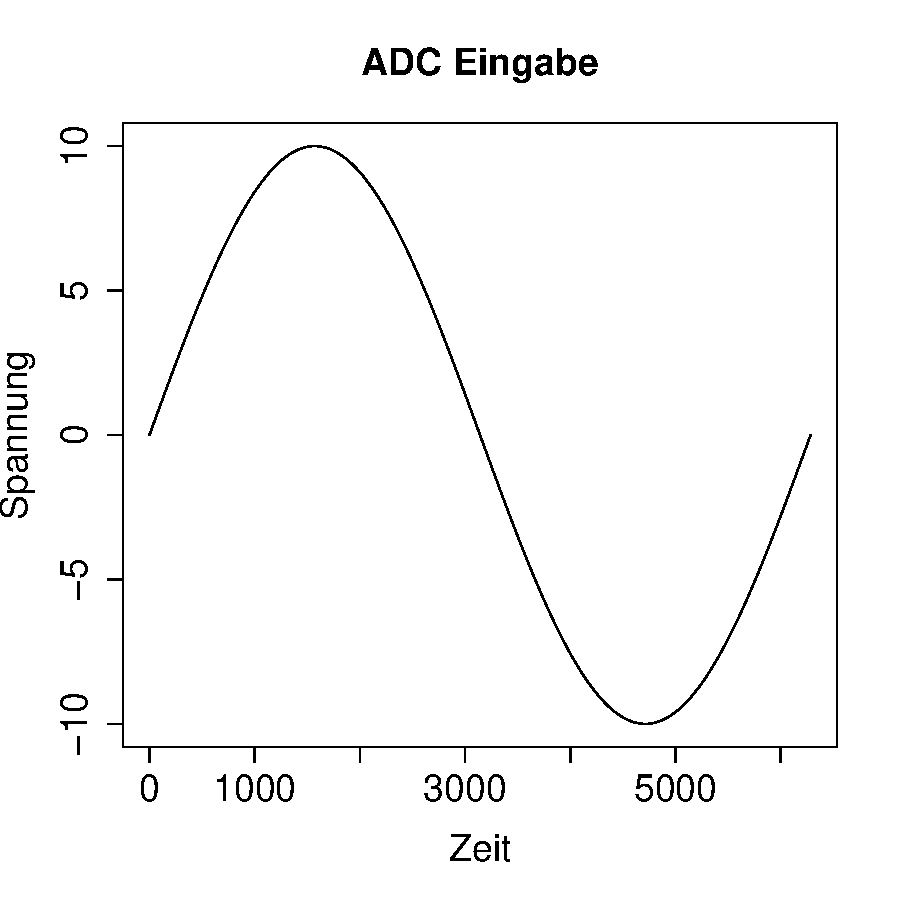
\includegraphics{verteilungen-065}
\caption{Eingangssignal $u_e(t)\in\mathbb{R}$}
\end{subfigure}
\begin{subfigure}[b]{0.48\textwidth}
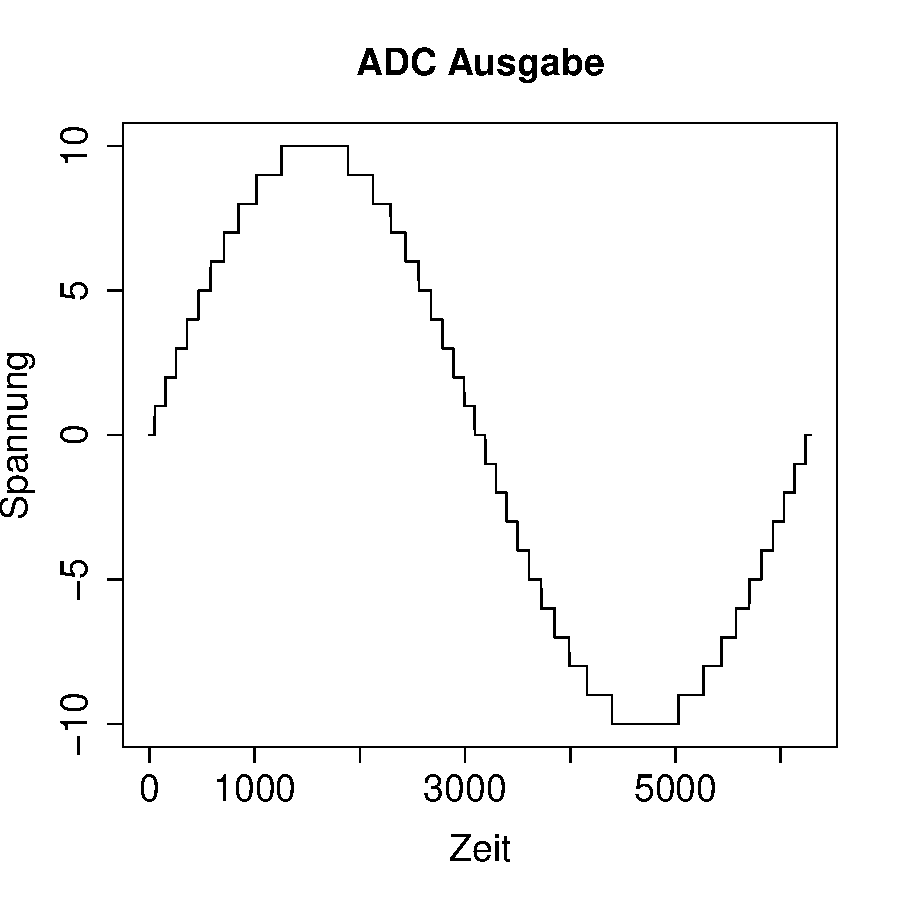
\includegraphics{verteilungen-066}
\caption{Digitalisierung $(\mathbb{R} \rightarrow 2^n, n\in \mathbb{N})$}
\end{subfigure}

\begin{subfigure}[b]{0.48\textwidth}
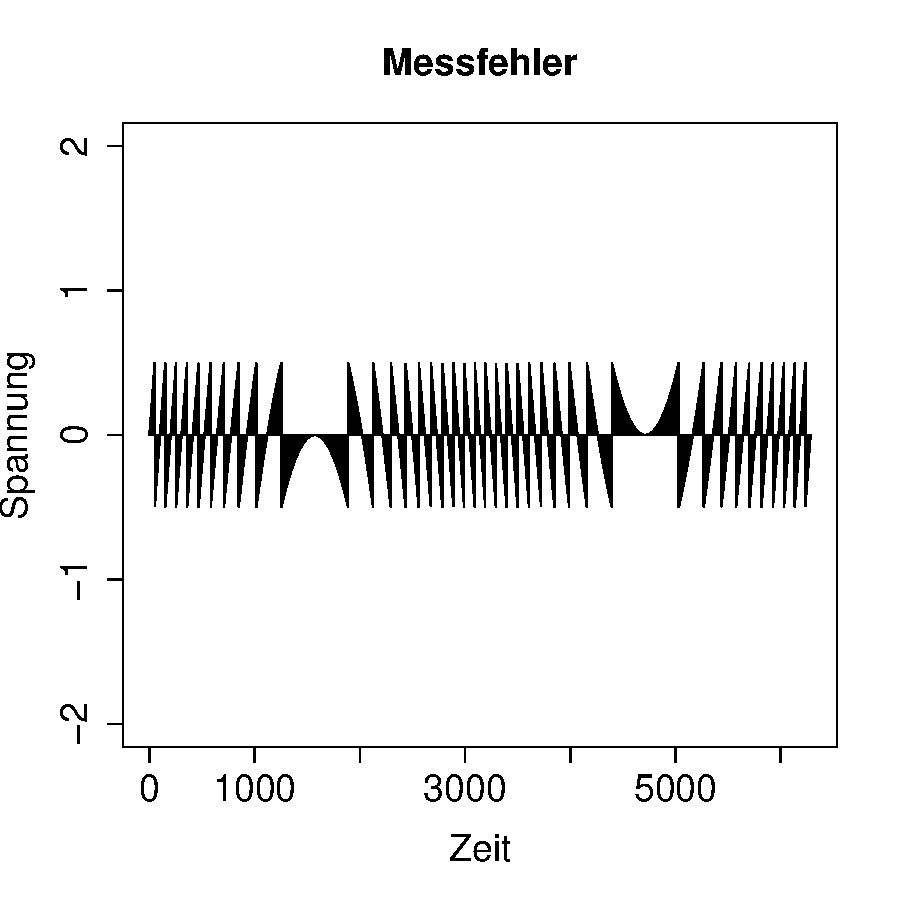
\includegraphics{verteilungen-067}
\caption{Fehler $u_a(t)$}
\end{subfigure}
\begin{subfigure}[b]{0.48\textwidth}
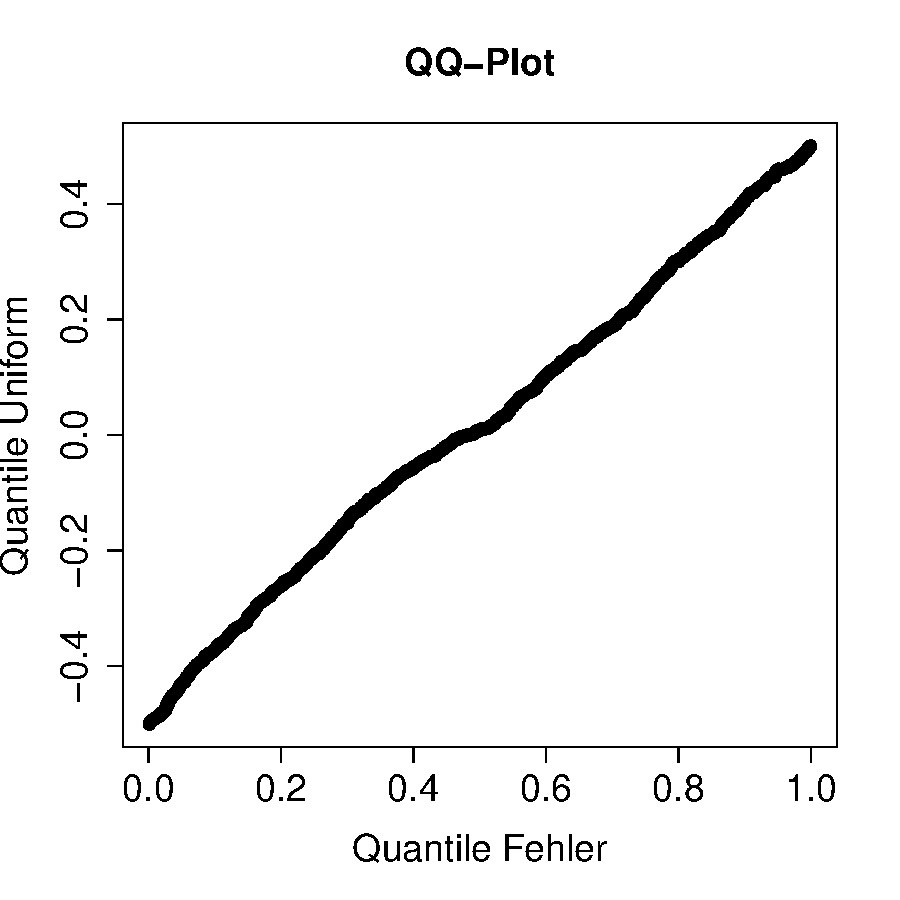
\includegraphics{verteilungen-068}
\caption{Quantilenvergleich mit $\mathcal{U}(a,b)$}
\label{fig:adc-d}
\end{subfigure}
\caption{Quantifizierungfehler eines ADC.}
\label{fig:adc}
\end{figure}

\newpage
\section{Normalverteilung}
Die Normalverteilung (auch \emph{Gauss-Verteilung} bzw. 
\emph{Gauss'sche Glockenkurve}) ist eine bedeutende stetige
Verteilung für sämtliche Bereiche der Natur- und 
Ingenieurwissenschaften. Der sog. \emph{Zentrale Grenzwertsatz}
macht sie zu einer der wichtigsten Verteilungen überhaupt
\parencite[297]{henze}. 


\[ 
	f(x) = \frac{1}{\sigma\sqrt{2\pi}}\cdot e^{
		\left( -\frac{(x-\mu)^2}{2\sigma^2} \right)}
\]

\begin{figure}[h!]
	\centering
	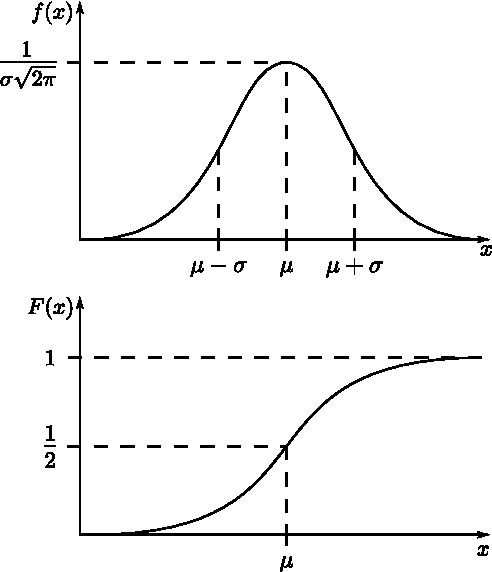
\includegraphics[width=0.7\textwidth]{normal.pdf}
	\caption{Normalverteilung}
	\label{fig:normal}
\end{figure}

\noindent
Der Zentrale Grenzwertsatz besagt,
dass ein Stichprobenmittelwert $\overline{x}$ für grosse
Stichproben annähernd normalverteilt ist mit 
$\overline{X}\sim\mathcal{N}(\mu, \frac{\sigma^2}{n})$ 
wobei der kritische Stichprobenumfang bei ca. 30 Stichproben
liegt \parencite[481]{oreilly}.


Die Interpretation der Normalverteilung 
$X \sim \mathcal{N}(\mu, \sigma^2)$
ist sehr anschaulich durch deren Parameter. Der Mittelwert 
$\mu$ zeigt das Zentrum der \emph{Glockenkurve} an, wo auch die 
Wahrscheinlichkeit am höchsten ist. Die Varianz zeigt an, wie 
flach die \emph{Glockenkurve} ist. 

Ein Spezialfall der Normalverteilung ist die sog.
\emph{standardisierte Normalverteilung}, welche einen 
Erwartungswert $\mu=0$ und eine Varianz $\sigma^2=1$ hat.
Mittels dieser lassen sich Ergebnisse beliebig transformieren
\parencite[298]{henze}.


\subsection{Verteilungsfunktion}

\subsection{Erwartungswert}
Der Erwartungswert einer Normalverteilung beschreibt jene
Stelle $x$ bei der die \emph{Glockenkurve} am höchsten ist.
Dieser Wert ist zugleich auch ein Parameter der Dichtefunktion
der Normalverteilung.
\[  
	E(X) = \mu
\]

\subsection{Varianz}
Die Varianz einer Normalverteilung ist wie der Erwartungswert
$\mu$ gleich ein Parameter der Dichtefunktion und beschreibt
wie flach die \emph{Glockenkurve} ist.
\[  
	Var(X) = \sigma^2
\]

\subsection{Verwendung in R}
\lstinline{R} stellt grundsätzlich vier Funktionen für die 
Normalverteilung zur Verfügung. 
\begin{itemize}
	\item \lstinline{dnorm()} \hfill{} 
		(\emph{Wahrscheinlichkeitsverteilung})
	\item \lstinline{pnorm()} \hfill{}
		(\emph{kumulative Wahrscheinlichkeit})
	\item \lstinline{qnorm()} \hfill{}
		(\emph{Verteilung der Quantile})
	\item \lstinline{rnorm()} \hfill{}
		(\emph{Zufallszahlen})
\end{itemize}
Die Abbildung \ref{fig:norm} zeigt jeweils einen Plot zu den gegebenen
Funktionen aus \lstinline{R}. Für weitere Informationen zu Plots siehe
Kapitel \ref{sec:plots}.





\begin{figure}[h!]
\centering
\begin{subfigure}[b]{0.48\textwidth}
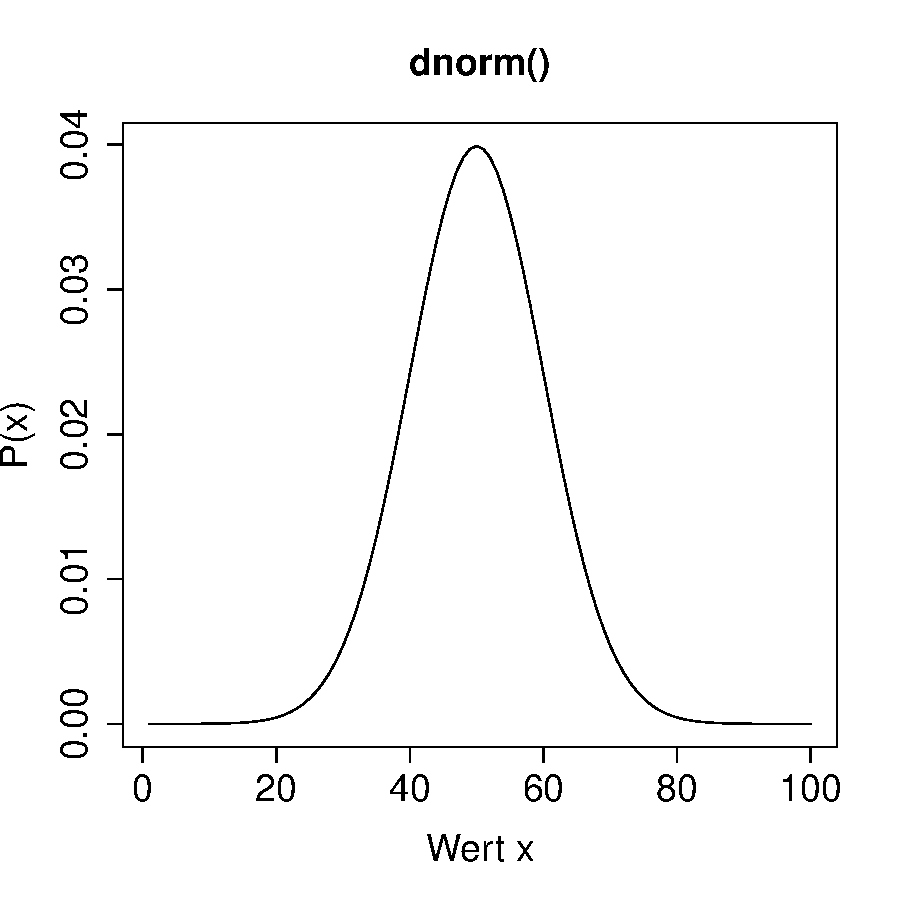
\includegraphics{verteilungen-073}
\caption{Wahrscheinlichkeitsverteilung}
\end{subfigure}
\begin{subfigure}[b]{0.48\textwidth}
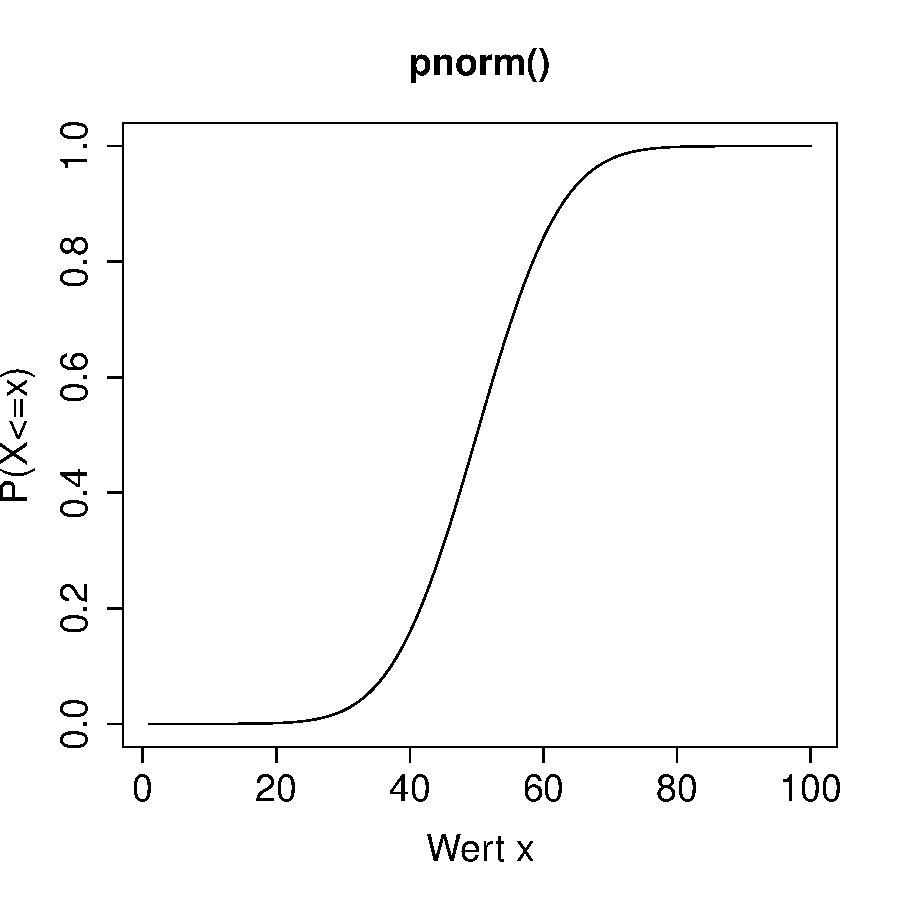
\includegraphics{verteilungen-074}
\caption{kumulative Wahrscheinlichkeit}
\end{subfigure}

\begin{subfigure}[b]{0.48\textwidth}
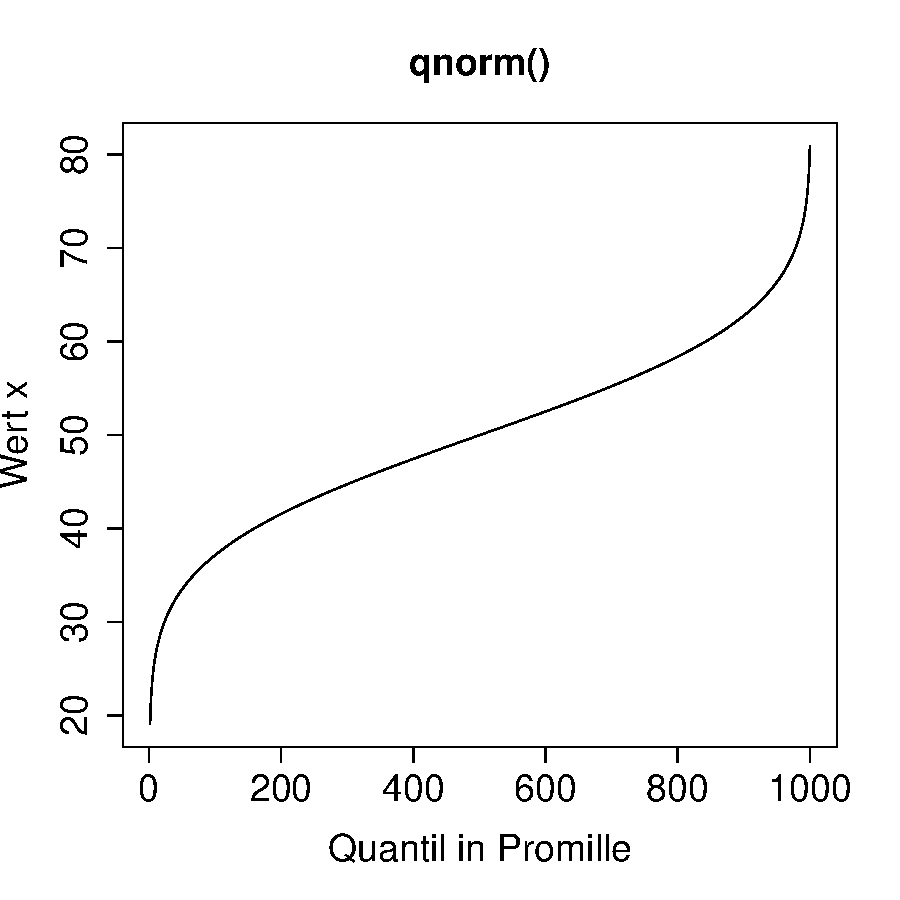
\includegraphics{verteilungen-075}
\caption{Quantile}
\end{subfigure}
\begin{subfigure}[b]{0.48\textwidth}
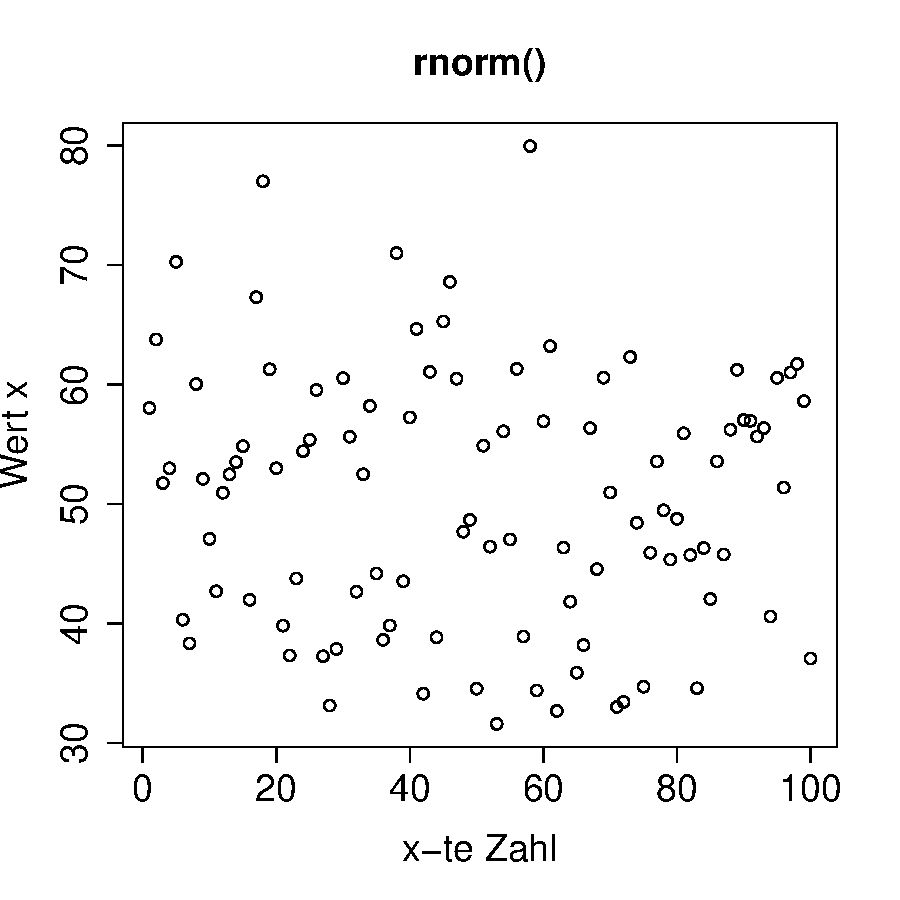
\includegraphics{verteilungen-076}
\caption{Zufallszahlen}
\end{subfigure}
\caption{Normalverteilung ($\mu=50, \sigma^2=10$)}
\label{fig:norm}
\end{figure}

\clearpage

\subsection{Beispiel einer Normalverteilung}
Bei digitalen Übertragungen entsteht durch diverse Umwelteinflüsse 
ein sog. \emph{Jitter}. Dieser beschreibt ein variieren der 
Taktzeiten einer Übertragung. Ein Teil des gesamten Jitters bildet 
der sogenannte \emph{zufällige Jitter} welcher Normalverteilt ist.
D.h. die zeitliche Grenze eines Zyklus folgt einer bestimmten
Verteilung, wobei die Ränder dieser Grenzen normalverteilt abweichen.

\begin{figure}[h!]
	\centering
	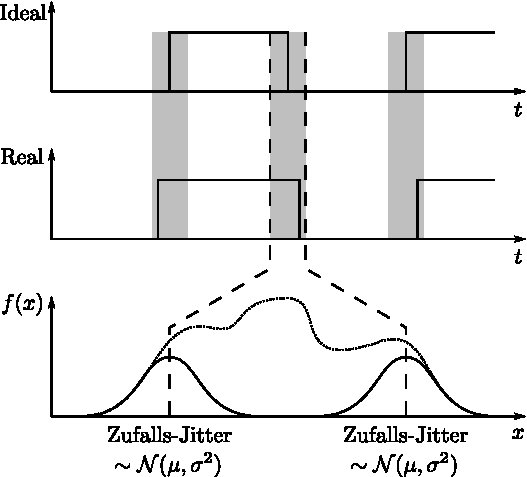
\includegraphics[width=0.7\textwidth]{jitter.pdf}
	\caption{Zufalls-Jitter}
	\label{fig:jitter}
\end{figure}

In vielen Anwendung von Mikrocontrollern  wird dieser Jitter ausführlich
beschrieben (siehe Anhang \ref{sec:stm32f21xx}).

\clearpage

\newpage
\section{Exponentialverteilung}
Die Exponentialverteilung (auch \emph{negative Exponentialverteilung}) ist 
eine stetige Verteilung welche angewandt wird um die Zeit beschreiben, welche
zwischen Ereignissen verstreicht. Dies gilt für Ereignisse  welche 
kontinuierlich, unabhängig und mit konstanter Rate ($\lambda$) eintreten.

\[  
	f(x) = \left\{ 
	\begin{array}{c c l}
		\displaystyle 
		\lambda \cdot e^{-\lambda \cdot x}
			& \text{falls}
			& x \geq 0 \\
		& & \\
		\displaystyle 
		0
			& \text{falls}
			& x < 0
	\end{array}
	\right.
\]

\begin{figure}[h!]
	\centering
	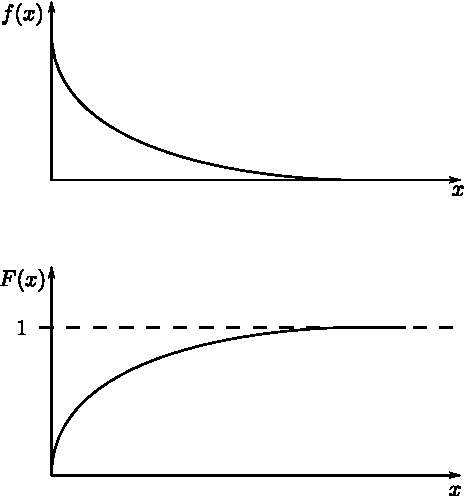
\includegraphics[width=0.7\textwidth]{exponential.pdf}
	\caption{Exponentialverteilung}
	\label{fig:exponential}
\end{figure}

Eine wichtige Eigenschaft der Exponentialverteilung ist die sog. 
\emph{Gedächtnislosigkeit} \parencite[296]{henze}. Diese besagt, dass die 
Wahrscheinlichkeit eines Ereignisses ab einem Zeitpunkt $t$ innerhalb des 
Intervalls $[a,b]$ nicht dadurch beeinflusst wird, ob und wann das letzte
Ereignis eingetreten ist.

\subsection{Verteilungsfunktion}
\[ 
	F(x) = \left\{ 
	\begin{array}{c c l}
		1-e^{-\lambda \cdot x}
			& \text{falls}
			& x \geq 0 \\
		& & \\
		0
			& \text{falls}
			& x < 0
	\end{array}
	\right.
\]

\subsection{Erwartungswert}
\[ 
	E(X) = \frac{1}{\lambda}
\]

\subsection{Varianz}
\[  
	Var(X) = \frac{1}{\lambda^2}
\]

\subsection{Standardabweichung}
Die Standardabweichung der Exponentialverteilung entspricht dem 
Erwartungswert.
\[  
	\sigma_x = \sqrt{\sigma^2} = \sqrt{Var(X)} = E(X) = \frac{1}{\lambda}
\]

\subsection{Transformation}
Die Verteilung $X \sim Exp(\lambda)$ mit beliebigem $\lambda \in \mathbb{R}$
kann aus der Grundform $X \sim Exp(1)$ transformeirt werden, denn die 
Änderung des Parameters bewirkt lediglich eine Skalenänderung 
\parencite[296]{henze}. Hierfür wird die Grundform mit dem reziproken Wert
des Parameters multipliziert.
\[  
	X \sim Exp(1) \Rightarrow \frac{1}{\lambda} \cdot X \sim Exp(\lambda)	
\]

\subsection{Zusammenhang mit uniformer Verteilung}
Die Exponentialverteilung hat einen direkten Zusammenhang mit der uniformen
Verteilung innerhalb des Intervalls $[0,1]$ mit 
$x \rightarrow -\frac{1}{\lambda} \cdot \log(1-x)$ und somit
\[  
	X \sim \mathcal{U}(0,1) 
		\Rightarrow 
		-\frac{1}{\lambda} \cdot \log(1-X) \sim Exp(\lambda)
\]
Mit diesem Zusammenhang lässt sich aus einer uniform verteilten Zufallszahl 
eine Exponentialverteilte Zufallszahl erzeugen \parencite[297]{henze}.

\subsection{Verwendung in R}
\lstinline{R} stellt grundsätzlich vier Funktionen für die 
Exponentialverteilung zur Verfügung. 
\begin{itemize}
	\item \lstinline{dexp()} \hfill{} 
		(\emph{Wahrscheinlichkeitsverteilung})
	\item \lstinline{pexp()} \hfill{}
		(\emph{kumulative Wahrscheinlichkeit})
	\item \lstinline{qexp()} \hfill{}
		(\emph{Verteilung der Quantile})
	\item \lstinline{rexp()} \hfill{}
		(\emph{Zufallszahlen})
\end{itemize}
Die Abbildung \ref{fig:exp} zeigt jeweils einen Plot zu den gegebenen
Funktionen aus \lstinline{R}. Für weitere Informationen zu Plots siehe
Kapitel \ref{sec:plots}.





\begin{figure}[h!]
\centering
\begin{subfigure}[b]{0.48\textwidth}
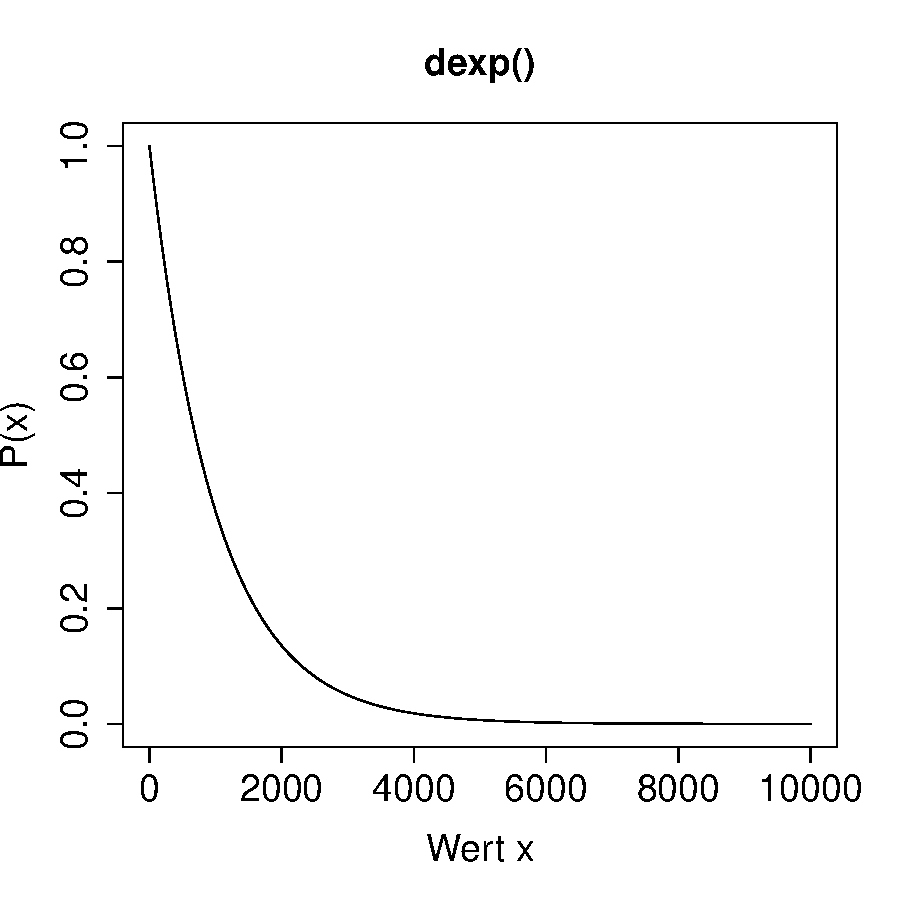
\includegraphics{verteilungen-081}
\caption{Wahrscheinlichkeitsverteilung}
\end{subfigure}
\begin{subfigure}[b]{0.48\textwidth}
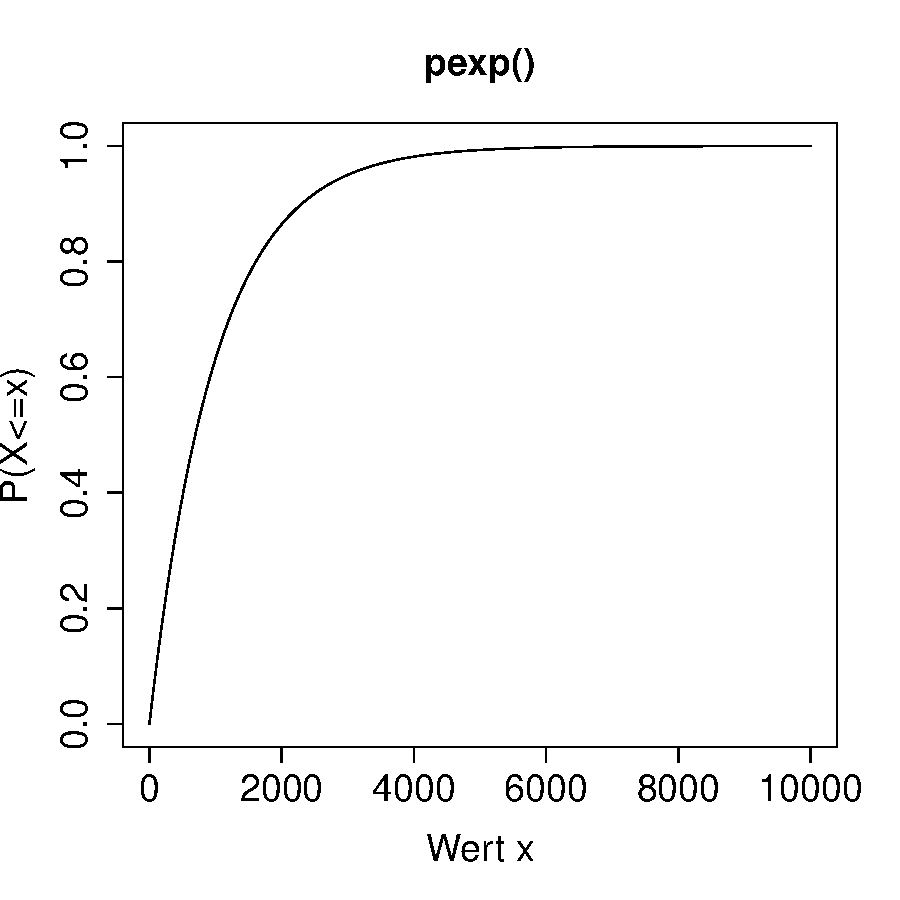
\includegraphics{verteilungen-082}
\caption{kumulative Wahrscheinlichkeit}
\end{subfigure}

\begin{subfigure}[b]{0.48\textwidth}
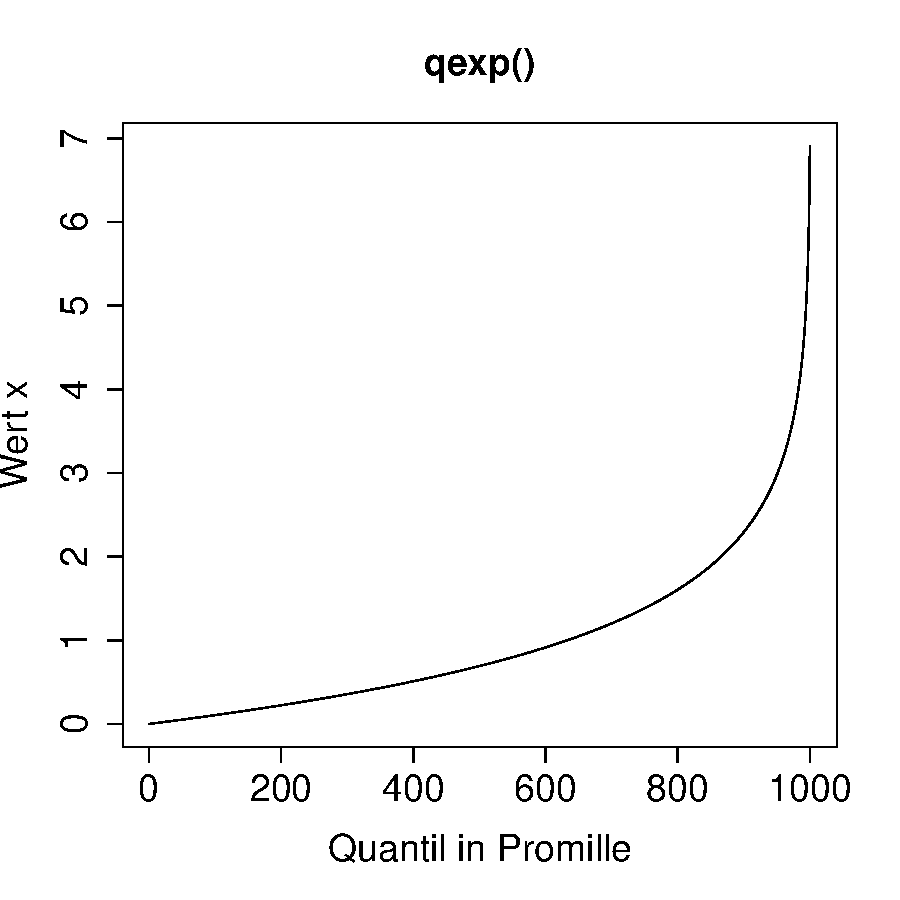
\includegraphics{verteilungen-083}
\caption{Quantile}
\end{subfigure}
\begin{subfigure}[b]{0.48\textwidth}
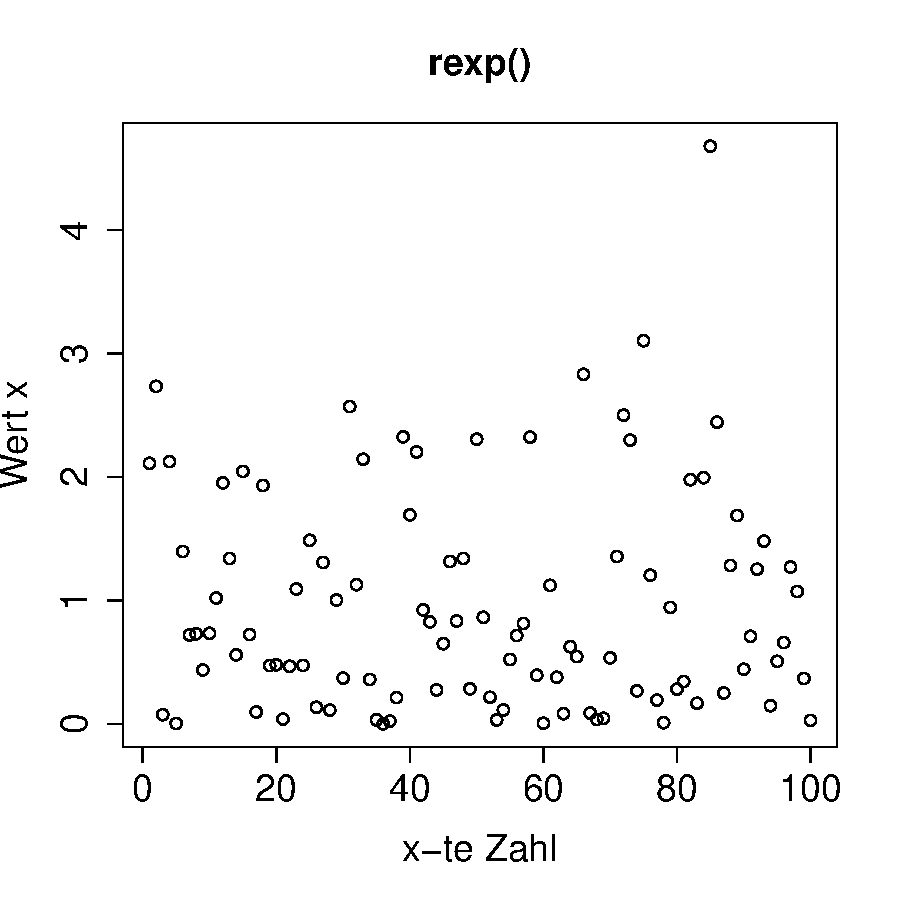
\includegraphics{verteilungen-084}
\caption{Zufallszahlen}
\end{subfigure}
\caption{Exponentialverteilung}
\label{fig:exp}
\end{figure}

\clearpage

\subsection{Beispiel einer Exponentialverteilung}
\paragraph{Beispiel 1 - Gerätedefekt}
Die Entwickler eines Sicherheitssystems möchten eine Gerätekomponente
einkaufen, statt diese selber zu entwicklen. Die favorisierte Komponente
hat laut Hersteller eine Ausfallrate von ca. $0.2\%$ pro Tag bei 
Dauerbetrieb.

Die Entwickler müssen nun folgende Frage beantworten für Ihren 
Entwicklungsbericht: "`\emph{Wie gross ist die Wahrscheinlichkeit, dass
die eingekaufte Komponente mindestens ein Jahr im Dauerbetrieb arbeitet?}"'

\begin{Schunk}
\begin{Sinput}
> dpd <- 0.002 # rate of defects per day
> ttd <- 1/dpd # time till defect
> ttd
\end{Sinput}
\begin{Soutput}
[1] 500
\end{Soutput}
\begin{Sinput}
> 1-pexp(q=365, rate=dpd)
\end{Sinput}
\begin{Soutput}
[1] 0.481909
\end{Soutput}
\end{Schunk}

\paragraph{Beispiel 2 - Reboot}
Der Administrator der Telefondatenbank der Firma Umbrella Corp. soll ein 
Update der Software machen. Hierzu muss der Service kurz abgestellt werden. 
Für den Reboot und das aufsarten des Service benötigt der Administrator ca. 
2 Minuten. 

Er überlegt sich nun, ob er den Reboot jetzt während den regulären 
Arbeitszeiten machen oder bis nach Feierabend warten soll. Da er nicht
sonderlich lust hat so lange im Betrieb zu sein, entschliesst er sich die
sache mal zu rechnen. Hierzu sieht er sich die Logfiles des Dienstes an und
bemerkt, dass ca. 15 Requests pro Stunde an den Dienst gehen. Also fragt er
sich nun: "`\emph{Wie wahrscheinlich ist es, dass ich innerhalb von zwei 
Minuten ab den Zeitpunkt $x$ einen Request erhalte?}"'

\begin{Schunk}
\begin{Sinput}
> rph <- 15 # requests per hour
> rt <- (1/30) # time for reboot and service start in hours
> pexp(q=rt, rate=rph)
\end{Sinput}
\begin{Soutput}
[1] 0.3934693
\end{Soutput}
\end{Schunk}

Bei Berechnungen von Exponentialverteilten Wahrscheinlichkeiten ist die 
sog. \emph{Gedächtnislosigkeit} der Verteilung zu beachten. Für das obige
Beispiel heisst dies, dass die Wahrscheinlichkeit eines Requests innert
der nächsten $x$ Minuten nicht davon beieinflusst wird, ob gerade eben
ein Request stattfand oder nicht.

\newpage
\section{Zusammenfassung}
\paragraph{Uniforme Verteilung}
\[ X \sim \mathcal{U}(a,b) \]
\[ \begin{array}{l c l}
	F(X) 
		& =
		& \displaystyle \frac{x-a}{b-a} \\
	f(x)	
		& =
		& \displaystyle \frac{1}{b-a}  \\
	D_f	
		& = 
		& a < x < b \\
	E(X)
		& = 
		& \displaystyle \frac{a+b}{2}\\
	Var(X)	
		& =
		& \displaystyle \frac{(b-a)^2}{12}\\
\end{array} \]

\paragraph{Normalverteilung}
\[ X \sim \mathcal{N}(\mu, \sigma^2) \]
\[ \begin{array}{l c l}
	F(X) 
		& =
		& \displaystyle \frac{x-a}{b-a} \\
	f(x)	
		& =
		& \displaystyle \frac{1}{\sigma\sqrt{2\pi}} \cdot
				e^{\left(
					-\frac{(x-\mu)^2}{2\sigma^2}
				\right)} \\
	D_f	
		& = 
		& x \in \mathbb{R} \\
	E(X)
		& = 
		& \mu\\
	Var(X)	
		& =
		& \sigma^2 \\
\end{array} \]

\paragraph{Exponentialverteilung}
\[ X \sim Exp(\lambda) \]
\[ \begin{array}{l c l}
	F(X) 
		& =
		& F(X) = \displaystyle \frac{x-a}{b-a} \\
	f(x)	
		& =
		& \displaystyle \lambda \cdot 
				e^{\left(
					-\lambda x
				\right)} \\
	D_f	
		& = 
		& x > 0 \\
	E(X)
		& = 
		& \displaystyle \frac{a+b}{2}\\
	Var(X)	
		& =
		& \displaystyle \frac{(b-a)^2}{12}\\
\end{array} \]


\subsection{Berechnungen in R}

\begin{table}[h!]
	\begin{tabular}{l l l}
	$X \sim \mathcal{U}(a,b)$ & & \\ %\hline
		& genau $A$ 		& \verb!dunif(x=A,...)! \\
		& höchstens $A$		& \verb!punif(q=A,...)! \\
		& mindestens $A$	& \verb!1-punif(q=A-1,...)! \\
		& $A$ zufällige 	& \verb!runif(n=A...)! \\
	& & \\
	$X \sim \mathcal{N}(\mu, \sigma^2)$ & & \\ %\hline
		& genau $A$		& \verb!dnorm(x=A,...)! \\
		& höchstens $A$		& \verb!pnorm(q=A,...)! \\
		& mindestens $A$	& \verb!1-pnorm(q=A-1,...)! \\
		& $A$ zufällige 	& \verb!rnorm(n=A...)! \\
	& & \\
	$X \sim Exp(\lambda)$ & & \\ %\hline
		& genau $A$		& \verb!dexp(x=A,...)! \\
		& höchstens $A$		& \verb!pexp(q=A,...)! \\
		& mindestens $A$	& \verb!1-pexp(q=A-1,...)! \\
		& $A$ zufällige 	& \verb!rexp(n=A...)! \\
	\end{tabular}
\end{table}
